%=============================================================================
% SRM Institute of Science and Technology
% Case Study Report for 21CSC406J – NEURAL NETWORKS AND DEEP LEARNING
% Development of Deep Learning Based Water Quality Deterioration Prediction Framework Using Temporal Sensor Data
% Authors: Kunwar Abhyansh Visen [RA2311026010576], Ayushmaan Krishna [RA2311026010570], Shashank A. Patil [RA2311026010573]
% Faculty Guide: Ms. Uma E
%=============================================================================

\documentclass[12pt,a4paper]{report}

%--- Packages ----------------------------------------------------------------
\usepackage[top=1in,bottom=1in,left=1in,right=1in]{geometry}
\usepackage{times}          % Times New Roman throughout
\usepackage{setspace}       % 1.5 line spacing
\usepackage{titlesec}       % Chapter/section heading formatting
\usepackage{titletoc}       % TOC formatting
\usepackage{tocloft}        % Fine-grained TOC/LOF/LOT control
\usepackage{fancyhdr}       % Headers and footers
\usepackage{graphicx}       % Figures
\usepackage{booktabs}       % Professional table rules
\usepackage{longtable}      % Multi-page tables
\usepackage{array}          % Column spec extensions
\usepackage{tabularx}       % Auto-width table columns
\usepackage{multirow}       % Multi-row cells
\usepackage{caption}        % Caption formatting
\usepackage{amsmath}        % Math
\usepackage{amssymb}        % Math symbols
\usepackage[round,authoryear]{natbib} % Author--date citations
\usepackage{hyperref}       % Hyperlinks (load last mostly)
\usepackage{url}            % URL formatting
\usepackage{enumitem}       % List customisation
\usepackage{indentfirst}    % Indent first paragraph of each section
\usepackage{parskip}        % Spacing between paragraphs
\usepackage{emptypage}      % Suppress headers on blank pages
\usepackage{microtype}      % Better justification
\usepackage{ragged2e}       % \justifying command
\usepackage{float}          % [H] placement specifier
\usepackage{needspace}      % Keep headings with the content that follows

%--- Font: Times New Roman everywhere ----------------------------------------
\renewcommand{\rmdefault}{ptm}
\renewcommand{\sfdefault}{phv}
\renewcommand{\ttdefault}{pcr}

%--- Line spacing -------------------------------------------------------------
\onehalfspacing

%--- Paragraph spacing --------------------------------------------------------
\setlength{\parskip}{6pt}
\setlength{\parindent}{0.5in}

%--- Text justification -------------------------------------------------------
\justifying

%--- Page style ---------------------------------------------------------------
\pagestyle{fancy}
\fancyhf{}
\fancyfoot[C]{\thepage}
\renewcommand{\headrulewidth}{0pt}

% Plain style for chapter-start pages
\fancypagestyle{plain}{
  \fancyhf{}
  \fancyfoot[C]{\thepage}
  \renewcommand{\headrulewidth}{0pt}
}

%--- Chapter heading format ---------------------------------------------------
\titleformat{\chapter}[display]
  {\centering\fontsize{20}{24}\selectfont\bfseries}
  {\MakeUppercase{\chaptertitlename}\ \thechapter}
  {0pt}
  {\MakeUppercase}
\titlespacing*{\chapter}{0pt}{0pt}{18pt}

%--- Section heading format ---------------------------------------------------
\titleformat{\section}
  {\raggedright\fontsize{16}{20}\selectfont\bfseries}
  {\thesection}
  {1em}
  {}
\titlespacing*{\section}{0pt}{16pt}{6pt}

%--- Subsection heading format ------------------------------------------------
\titleformat{\subsection}
  {\raggedright\fontsize{14}{18}\selectfont\bfseries}
  {\thesubsection}
  {1em}
  {}
\titlespacing*{\subsection}{0pt}{12pt}{4pt}

%--- Table caption above, Figure caption below --------------------------------
\captionsetup[table]{position=above, labelsep=colon,
  font={small,bf,it}, justification=centering, singlelinecheck=false}
\captionsetup[figure]{position=below, labelsep=colon,
  font={small,bf,it}, justification=centering}

%--- Table/Figure numbering: chapter.number -----------------------------------
\numberwithin{table}{chapter}
\numberwithin{figure}{chapter}

%--- TOC depth ----------------------------------------------------------------
\setcounter{tocdepth}{3}
\setcounter{secnumdepth}{3}

%--- Table of contents layout matching the supplied report template ------------
\newcolumntype{T}[1]{>{\centering\arraybackslash}p{#1}}

%--- Column type for fixed-width justified cells ------------------------------
\newcolumntype{L}[1]{>{\RaggedRight\arraybackslash}p{#1}}
\newcolumntype{C}[1]{>{\centering\arraybackslash}p{#1}}
\newcolumntype{R}[1]{>{\RaggedLeft\arraybackslash}p{#1}}

%--- Hyperref config ----------------------------------------------------------
\hypersetup{
  colorlinks=true,
  linkcolor=black,
  citecolor=black,
  urlcolor=black,
  pdfauthor={Kunwar Abhyansh Visen, Ayushmaan Krishna, Shashank A. Patil},
  pdftitle={Development of Deep Learning Based Water Quality Deterioration Prediction Framework Using Temporal Sensor Data},
}

%=============================================================================
\begin{document}
%=============================================================================

%--- Frontmatter page numbering (Roman) --------------------------------------
\pagenumbering{roman}

%=============================================================================
%  COVER PAGE
%=============================================================================
\begin{titlepage}
\centering
\vspace*{1.5cm}

{\fontsize{18}{22}\selectfont\bfseries
DEVELOPMENT OF DEEP LEARNING BASED WATER QUALITY DETERIORATION PREDICTION FRAMEWORK USING TEMPORAL SENSOR DATA\\[0.4cm]}

{\fontsize{16}{20}\selectfont\bfseries CASE STUDY REPORT\\[0.15cm]}
{\fontsize{14}{18}\selectfont for\\[0.2cm]}
{\fontsize{14}{18}\selectfont 21CSC406J \textendash\ NEURAL NETWORKS AND DEEP LEARNING\\[0.6cm]}

{\fontsize{14}{18}\selectfont Submitted by\\[0.3cm]}

{\fontsize{14}{18}\selectfont\itshape
Kunwar Abhyansh Visen \quad [RA2311026010576]\\[0.2cm]
Ayushmaan Krishna \quad [RA2311026010570]\\[0.2cm]
Shashank A. Patil \quad [RA2311026010573]\\[0.6cm]}

In partial fulfilment of the requirements for the degree of\\[0.4cm]

{\fontsize{14}{18}\selectfont\bfseries
BACHELOR OF TECHNOLOGY\\[0.15cm]
in\\[0.15cm]
COMPUTER SCIENCE ENGINEERING\\[0.15cm]
with specialization in AIML\\[0.6cm]}

{\fontsize{16}{20}\selectfont\bfseries
DEPARTMENT OF COMPUTATIONAL INTELLIGENCE\\
COLLEGE OF ENGINEERING AND TECHNOLOGY\\
SRM INSTITUTE OF SCIENCE AND TECHNOLOGY\\
KATTANKULATHUR -- 603\,203\\[0.5cm]}

{\fontsize{16}{20}\selectfont\bfseries NOVEMBER 2026}
\end{titlepage}

%=============================================================================
%  BONAFIDE CERTIFICATE
%=============================================================================
\newpage
\thispagestyle{plain}
\begin{center}
{\fontsize{18}{22}\selectfont\bfseries SRM INSTITUTE OF SCIENCE AND TECHNOLOGY\\
KATTANKULATHUR -- 603\,203\\[0.6cm]}
{\fontsize{16}{20}\selectfont\bfseries BONAFIDE CERTIFICATE\\[0.4cm]}
\end{center}

\noindent This is to certify that the Case Study Report titled ``\textbf{Development of Deep Learning Based Water Quality Deterioration Prediction Framework Using Temporal Sensor Data}'' is a bonafide record of work carried out by the following student(s) as part of the course 21CSC406J -- NEURAL NETWORKS AND DEEP LEARNING, during the academic year 2026--2027 Odd Semester:

\vspace{0.3cm}
\noindent Submitted by:

\begin{center}
\renewcommand{\arraystretch}{1.25}
\begin{tabular}{|c|l|}
\hline
\textbf{Register Number} & \textbf{Name of Student(s)} \\
\hline
RA2311026010576 & Kunwar Abhyansh Visen \\
\hline
RA2311026010570 & Ayushmaan Krishna \\
\hline
RA2311026010573 & Shashank A. Patil \\
\hline
\end{tabular}
\end{center}

This report has been submitted in partial fulfilment of the requirements for the successful completion of the course and has not been submitted elsewhere for any academic or non-academic purpose.

The work is found to be satisfactory and is hereby accepted.

\vspace{0.8cm}
\noindent\begin{tabular}{@{}p{7cm} @{}p{7cm}}
\textbf{Ms. Uma E} & \textbf{Dr. R. Annie Uthra} \\
Supervisor, Faculty Guide & Professor \& Head \\
Department of Computational Intelligence & Department of Computational Intelligence \\
SRMIST, KTR & SRMIST, KTR \\
\end{tabular}

\vspace{0.8cm}
\noindent Date of Submission: \underline{\hspace{4cm}}

%=============================================================================
%  ABSTRACT
%=============================================================================
\newpage
\thispagestyle{plain}
\begin{center}
{\fontsize{14}{18}\selectfont\bfseries ABSTRACT\\[0.4cm]}
\end{center}
\addcontentsline{toc}{chapter}{ABSTRACT}

\noindent Water quality deterioration poses significant risks to public health and environmental sustainability across India. With thousands of surface water monitoring stations under the National Water Quality Monitoring Programme (NWMP), the challenge of timely and accurate deterioration prediction is immense. Conventional monitoring relies on manual sampling and laboratory testing, resulting in delayed responses to contamination events.

This work presents a Deep Learning Based Water Quality Deterioration Prediction Framework Using Temporal Sensor Data using the project dataset described as National Water Quality Monitoring Programme (NWMP) data from the Central Pollution Control Board (CPCB), covering 2019--2023. After preprocessing, the notebook records 1,990 labeled station-year samples, split into 1,500 training samples and 490 test samples. The core model is a TabTransformer-based architecture that learns feature interactions through multi-head self-attention.

The model classifies water samples into three categories (Safe, Marginal, Unsafe) according to BIS IS 10500:2012 standards, using 17 engineered features including physicochemical parameters (BOD, Nitrate, Total Coliform, DO, pH, Conductivity, Fecal Coliform, Temperature) and engineered spatio-temporal features (WQI Lag-1, WQI Rolling-3, WQI Trend, Pollution Growth Rate, Station Average WQI, State Average WQI, Station Violation Rate, WQI Deviation from State).

The recorded model comparison reports a Macro F1-score of 88.27\% for the TabTransformer on the 490-sample test set, compared with 66.26\% for XGBoost and Random Forest. Test labels comprise 2 Safe, 139 Marginal, and 349 Unsafe samples. Since there are only two Safe examples in the test split, conclusions about Safe-class performance are preliminary.

The framework includes comprehensive explainability through SHAP GradientExplainer, identifying Total Coliform (0.412 mean |SHAP|), BOD (0.318), and Station Violation Rate (0.241) as the top deterioration drivers. A 30-iteration bootstrap framework provides per-sample confidence intervals (mean 99.0\%). A rule-based remediation engine maps top pollutants to tiered interventions across three time horizons (Immediate: 0-48hrs, Short-term: 1-3 months, Long-term: 1+ years).

A prototype decision-support dashboard integrates multi-horizon forecasting, deterioration risk scoring, seasonal analysis, and change-point detection. Dashboard outputs are prototype predictions and are distinct from the held-out classification evaluation described above.

\vspace{0.4cm}
\noindent\textbf{Keywords:} \textit{Water quality deterioration; deep learning; TabTransformer; temporal sensor data; SHAP; decision support; class imbalance; BIS IS 10500:2012; temporal forecasting; seasonal decomposition}

%=============================================================================
%  TABLE OF CONTENTS
%=============================================================================
\newpage
\thispagestyle{plain}
\begin{center}
  {\fontsize{14}{18}\selectfont\bfseries TABLE OF CONTENTS\\[0.5cm]}
\end{center}
\begingroup
\renewcommand{\arraystretch}{1.35}
\noindent\begin{tabularx}{\textwidth}{|T{3cm}|X|T{2cm}|}
\hline
\textbf{CHAPTER NO} & \centering\arraybackslash\textbf{TITLE} & \textbf{Page No} \\
\hline
1 & INTRODUCTION & \pageref{ch:introduction} \\
\hline
2 & THEORETICAL FOUNDATION: CNN, TRANSFER LEARNING, ATTENTION \& GANs & \pageref{ch:theory} \\
\hline
3 & CASE ANALYSIS \& IMPLEMENTATION & \pageref{ch:case-analysis} \\
\hline
4 & PROPOSED IMPROVEMENTS / OPTIMIZATION STRATEGIES & \pageref{ch:improvements} \\
\hline
5 & CONCLUSION AND FUTURE WORK & \pageref{ch:conclusion} \\
\hline
 & REFERENCES & \pageref{sec:references} \\
\hline
 & APPENDIX A: CODING & \pageref{app:coding} \\
\hline
\end{tabularx}
\endgroup

%=============================================================================
%  LIST OF FIGURES
%=============================================================================
\newpage
\thispagestyle{plain}
\begin{center}
  {\fontsize{14}{18}\selectfont\bfseries LIST OF FIGURES\\[0.5cm]}
\end{center}
\begingroup
\renewcommand{\arraystretch}{1.35}
\noindent\begin{tabularx}{\textwidth}{|T{3.2cm}|T{2.6cm}|X|T{1.8cm}|}
\hline
\textbf{CHAPTER NO} & \textbf{FIG. NO} & \centering\arraybackslash\textbf{TITLE} & \textbf{Page No} \\
\hline
1 & \ref{fig:architecture} & System architecture overview & \pageref{fig:architecture} \\
\hline
3 & \ref{fig:remediation_panel} & Remediation engine output for Station 1263 & \pageref{fig:remediation_panel} \\
\hline
\end{tabularx}
\endgroup

%=============================================================================
%  LIST OF TABLES
%=============================================================================
\newpage
\thispagestyle{plain}
\begin{center}
  {\fontsize{14}{18}\selectfont\bfseries LIST OF TABLES\\[0.5cm]}
\end{center}
\begingroup
\renewcommand{\arraystretch}{1.35}
\noindent\begin{tabularx}{\textwidth}{|T{3.2cm}|T{2.9cm}|X|T{1.8cm}|}
\hline
\textbf{CHAPTER NO} & \textbf{TABLE. NO} & \centering\arraybackslash\textbf{TITLE} & \textbf{Page No} \\
\hline
2 & \ref{tab:litreview} & Summary of Existing Water Quality Machine Learning Models & \pageref{tab:litreview} \\
\hline
2 & \ref{tab:gaps} & Research Gaps Identified and How This Work Addresses Each & \pageref{tab:gaps} \\
\hline
3 & \ref{tab:modelcomp} & Comparative Performance on 2023 Test Set ($N=490$) & \pageref{tab:modelcomp} \\
\hline
3 & \ref{tab:remediation} & Remediation Engine -- Pollutant-to-Action Mapping by Time Horizon & \pageref{tab:remediation} \\
\hline
\end{tabularx}
\endgroup

%=============================================================================
%  MAIN BODY -- Arabic page numbering starts at Chapter 1
%=============================================================================
\newpage
\pagenumbering{arabic}
\setcounter{page}{1}

%=============================================================================
%  CHAPTER 1: INTRODUCTION
%=============================================================================
\chapter{INTRODUCTION}
\label{ch:introduction}

\section{Background}

Water quality deterioration poses a critical threat to public health and environmental sustainability in India. With over 4,000 surface water monitoring stations under the National Water Quality Monitoring Programme (NWMP) operated by the Central Pollution Control Board (CPCB), the challenge of timely and accurate deterioration prediction is immense. Conventional monitoring relies on manual sampling, laboratory testing, and expert review -- a process inherently slow, costly, and unresponsive to real-time contamination events.

This report presents a water quality classification framework using the project dataset described as CPCB/NWMP records from 2019--2023. The processed dataset contains 1,990 labeled station-year samples, including a 490-sample held-out test split. The core model is a TabTransformer-based architecture that learns feature interactions through multi-head self-attention.

The model classifies water samples into three categories (Safe, Marginal, Unsafe) according to BIS IS 10500:2012 standards, using 17 engineered features including 8 physicochemical parameters and 9 engineered spatio-temporal features. The framework integrates comprehensive explainability through SHAP, confidence quantification via bootstrap, and a rule-based remediation engine with tiered interventions.

\begin{figure}[H]
    \centering
    \includegraphics[scale=0.1]{images/architecture.png}
    \caption{System architecture overview.}
    \label{fig:architecture}
\end{figure}

\section{Problem Statement}

Conventional water quality surveillance in India relies on manual sampling, laboratory testing, and expert review -- a process inherently slow, costly, and unresponsive to real-time contamination events. Existing machine learning solutions in this domain are plagued by three key shortcomings: (1) they optimize for raw accuracy without accounting for severe class imbalance between Safe, Marginal, and Unsafe samples; (2) they discard spatial and temporal context inherent in multi-year station-level sensor data; (3) they provide no interpretable output for regulators who must act on the results.

A predictive model that labels every sample as Unsafe can achieve high raw accuracy while remaining operationally useless. This project addresses how a BIS-threshold-based classifier can account for class imbalance, provide interpretable predictions, and support actionable remediation. The implemented classification model uses station and temporal features; forecasting and other time-series analyses are presented as prototype decision-support capabilities rather than as the evaluated classifier task.

\section{Objectives}

The key objectives of this project are:

\begin{enumerate}[leftmargin=1.5cm]
  \item Develop a water quality deterioration prediction framework that is regulatory-compliant with BIS IS 10500:2012 standards.
  \item Evaluate performance under severe class imbalance using Macro F1 alongside accuracy.
  \item Incorporate spatial and temporal context from multi-year station-level sensor data.
  \item Provide interpretable output using SHAP-based explanations for regulatory acceptance.
  \item Generate actionable remediation plans from predictions.
  \item Integrate prototype multi-horizon forecasting and uncertainty displays in the decision-support dashboard.
\end{enumerate}

%=============================================================================
%  CHAPTER 2: THEORETICAL FOUNDATION: CNN, TRANSFER LEARNING, ATTENTION & GANs
%=============================================================================
\chapter{THEORETICAL FOUNDATION: CNN, TRANSFER LEARNING, ATTENTION \& GANs}
\label{ch:theory}

\section{Convolutional Neural Networks (CNN)}

Convolutional Neural Networks form the backbone of modern computer vision and have been
adapted for time-series analysis through 1D convolutions. In water quality prediction,
CNNs can extract local temporal patterns from sensor sequences. The key operations
include convolution, pooling, and fully connected layers. For temporal sensor data,
1D-CNNs can extract local temporal dependencies with fewer parameters than recurrent
architectures. Dilated convolutions further expand the receptive field without
increasing parameter count, enabling capture of long-range temporal dependencies in
water quality sensor streams.

\section{Transfer Learning}

Transfer learning leverages pre-trained models on large datasets to bootstrap
performance on target tasks with limited data. In water quality prediction, models
pre-trained on large-scale environmental datasets (e.g., global water quality
repositories, satellite imagery) can be fine-tuned for specific regional monitoring
stations. Feature extraction layers from pre-trained CNNs or Transformers capture
generic water quality patterns (seasonal cycles, pollution signatures), while the
final classification head adapts to local BIS IS 10500:2012 thresholds. This approach
is particularly valuable for stations with limited historical data, where training
from scratch would overfit.

\section{Attention Mechanisms}

Attention mechanisms enable models to dynamically weight the importance of different
input elements. In the context of water quality deterioration prediction:

\textbf{Scaled Dot-Product Attention} computes attention weights as:
\begin{equation}
  \text{Attention}(Q,K,V) = \text{softmax}\left(\frac{QK^T}{\sqrt{d_k}}\right)V
\end{equation}
where $Q$, $K$, $V$ are query, key, and value matrices.

\textbf{Multi-Head Attention} projects queries, keys, and values into multiple
subspaces, enabling the model to attend to different feature interactions
simultaneously. The TabTransformer applies this across feature embeddings, learning
which water quality parameters interact to drive deterioration (e.g., BOD $\times$
Total Coliform interaction).

\textbf{Temporal Attention} extends attention across time steps, allowing the model
to focus on critical historical periods (e.g., monsoon onset, industrial discharge
events) when predicting deterioration.

\section{Generative Adversarial Networks (GANs)}

GANs consist of a generator $G$ and discriminator $D$ trained adversarially:
\begin{equation}
  \min_G \max_D \mathbb{E}_{x \sim p_{data}}[\log D(x)] + \mathbb{E}_{z \sim p_z}[\log(1-D(G(z)))]
\end{equation}
In water quality applications, GANs can:
\begin{itemize}
  \item \textbf{Data Augmentation}: Generate synthetic water quality samples for rare
    classes (Safe) to address class imbalance
  \item \textbf{Anomaly Detection}: Train discriminator to identify anomalous sensor
    readings that deviate from learned normal patterns
  \item \textbf{Missing Data Imputation}: Generator learns to impute missing sensor
    values conditioned on observed parameters
\end{itemize}
Conditional GANs (cGANs) can generate water quality samples conditioned on station
metadata (location, water body type) and temporal context (season, weather).

\section{Transformer Architectures for Tabular Data}

The \textbf{TabTransformer}~\cite{huang2020} applies multi-head self-attention to
categorical feature embeddings. Each feature is embedded into a $d$-dimensional space,
then refined through $L$ transformer encoder layers:
\begin{equation}
  Z_l = \operatorname{TransformerEncoderLayer}(Z_{l-1})
\end{equation}
The resulting contextual embeddings capture feature-feature interactions critical
for water quality deterioration (e.g., BOD $\times$ Total Coliform synergy).

The \textbf{FT-Transformer}~\cite{gorishniy2021} introduces per-feature tokenizers
(separate linear projections per feature) and a learnable [CLS] token for
classification. This architecture outperforms standard Transformers on tabular data
by preserving feature-specific information.

\section{SHAP Explainability Theory}

SHAP (SHapley Additive exPlanations)~\cite{lundberg2017} provides theoretically
grounded feature attribution via Shapley values from cooperative game theory:
\begin{equation}
  \phi_i = \sum_{S \subseteq F \setminus \{i\}} \frac{|S|!(|F|-|S|-1)!}{|F|!}
  [f(S \cup \{i\}) - f(S)]
\end{equation}
where $F$ is the set of all features. The SHAP GradientExplainer approximates
Shapley values using expected gradients, enabling efficient computation for deep
learning models. This provides both global feature importance (beeswarm plots) and
local sample-level explanations (waterfall plots).

\section{Temporal Forecasting and Seasonal Decomposition}

\textbf{STL Decomposition} (Seasonal-Trend decomposition using LOESS) separates a
time series into three components:
\begin{equation}
  y_t = T_t + S_t + R_t
\end{equation}
where $T_t$ is trend, $S_t$ is seasonal, and $R_t$ is residual. STL uses LOESS
smoothing for robust decomposition even with outliers common in sensor data.

\textbf{Fourier Analysis} decomposes signals into sinusoidal components:
\begin{equation}
  X_k = \sum_{n=0}^{N-1} x_n e^{-i 2\pi k n / N}
\end{equation}
For water quality, dominant frequencies reveal seasonal cycles (annual, semi-annual)
and potential anthropogenic periodicities (weekly industrial cycles).

\textbf{Multi-Horizon Forecasting} extends predictions to multiple future time steps.
Direct multi-horizon strategies train separate models for each horizon, while
recursive strategies use autoregressive generation. Uncertainty quantification via
prediction intervals (e.g., conformal prediction, bootstrap) is essential for
regulatory decision-making.

\section{Related Work and Research Gaps}

Table~\ref{tab:litreview} presents a comparative summary of key prior works.

\vspace{0.3cm}
\begin{table}[ht]
\caption{Summary of Existing Water Quality Machine Learning Models}
\label{tab:litreview}
\centering
\small
\begin{tabular}{@{} L{2.0cm} L{2.0cm} L{1.8cm} L{2.2cm} L{1.8cm} L{2.4cm} @{}}
\toprule
\textbf{Reference} & \textbf{Method} & \textbf{Task} & \textbf{Dataset / Region} & \textbf{Key Metric} & \textbf{Limitation} \\
\midrule
Chen et al.~\cite{chen2020}         & RF + ANN Ensemble        & WQ Prediction       & Surface water, China      & $R^2 > 0.90$      & No minority-class handling \\
Ahmed et al.~\cite{ahmed2019}       & Hybrid ML (SVM, RF)      & DO / BOD Prediction & Multiple regions          & RMSE improved     & Single-parameter focus \\
Ding et al.~\cite{ding2023}         & ML-based WQI             & Index Prediction    & Multi-body, China         & Improved weights  & No classification output \\
Wang et al.~\cite{wang2023}         & XGBoost + entropy FS     & WQI Prediction      & India surface water       & High accuracy     & Ignores temporal lag \\
Singha et al.~\cite{singha2021}     & Deep Learning            & Groundwater Quality & India                     & $R^2 >$ XGBoost   & No SHAP explanation \\
Li et al.~\cite{li2023}             & Multivariate LSTM        & DO / N Series       & River basins              & $R^2$: 0.82--0.86 & No classification task \\
Nallakaruppan et al.~\cite{nalla2024} & XAI + Ensemble         & WQ Classification   & Multi-source              & Macro F1: $\sim$72\% & No Safe-class detection \\
Shams et al.~\cite{shams2024}       & Multiple ML (Grid Search)& WQI Classification  & Benchmark datasets        & Accuracy: $\sim$89\% & No BIS compliance \\
\textbf{This Work}                  & \textbf{TabTransformer + SHAP} & \textbf{3-class BIS} & \textbf{India CPCB 2019--23} & \textbf{Macro F1: 88.27\%} & --- \\
\bottomrule
\end{tabular}
\end{table}
\centering

\section{Research Gaps Identified}

A systematic review reveals key gaps this work addresses:
\begin{enumerate}
  \item No existing system combines regulatory-compliant classification (BIS IS 10500:2012), deep tabular learning, gradient explainability, uncertainty quantification, and a remediation engine under a single framework.
  \item Class imbalance treatment is inadequate; most systems optimize for raw accuracy, missing the rare Safe class.
  \item Existing ML systems lack interpretable dashboards for regulators.
  \item Temporal forecasting with uncertainty quantification is absent from deployed systems.
  \item Seasonal decomposition and change point detection for deterioration monitoring are missing.
\end{enumerate}

Table~\ref{tab:gaps} maps each identified gap to the corresponding design choice.

\begin{table}[H]
\caption{Research Gaps Identified and How This Work Addresses Each}
\label{tab:gaps}
\centering
\footnotesize
\renewcommand{\arraystretch}{0.9}
\setlength{\tabcolsep}{3pt}
\begin{tabular}{@{} L{3.5cm} L{4.5cm} L{5.0cm} @{}}
\toprule
\textbf{Gap Identified} & \textbf{Observed in Literature} & \textbf{Addressed in This Work} \\
\midrule
No BIS IS 10500:2012 alignment       & Most models use WHO/EPA or no regulatory standard         & Labels generated directly from BIS thresholds; worst-case rule applied \\
Ignores class imbalance              & Raw accuracy used despite 70/25/5 class split             & Weighted Cross-Entropy Loss inversely proportional to class frequency \\
No spatio-temporal context           & Models use point-in-time values only                      & Lag features, rolling means, per-station violation rates engineered \\
Rare Safe-class examples            & Only three Safe labels appear in the full processed dataset & Report class-wise results with the small support stated explicitly \\
No interpretability                  & Black-box outputs with no feature attribution             & SHAP GradientExplainer provides global and local explanations \\
No uncertainty quantification        & Single point prediction with no confidence                & 30-iteration bootstrap gives per-sample confidence score \\
No remediation output                & Predictions not translated to actions                     & Rule-based engine maps top pollutants to tiered interventions \\
\bottomrule
\end{tabular}
\end{table}
\centering

\Needspace{6\baselineskip}
\section{Research Objectives}

Based on the identified gaps, the following research objectives were formulated:

\begin{enumerate}[leftmargin=1.5cm,itemsep=0pt,topsep=0pt,parsep=0pt]
  \item Develop a TabTransformer-based multi-class classification system aligned with BIS IS 10500:2012 standards.
  \item Engineer spatio-temporal features to capture temporal autocorrelation in station-level data.
  \item Address class imbalance using weighted Cross-Entropy Loss and evaluate with Macro F1-score.
  \item Apply SHAP GradientExplainer to provide global feature importance and local sample-level explanations.
  \item Implement a 30-iteration bootstrap framework to quantify prediction confidence.
  \item Build a rule-based remediation engine that maps pollutant-driven predictions to tiered, actionable interventions.
  \item Deploy a prototype decision-support dashboard integrating all components for operational use.
\end{enumerate}

%=============================================================================
%  CHAPTER 3: CASE ANALYSIS & IMPLEMENTATION
%=============================================================================
\chapter{CASE ANALYSIS \& IMPLEMENTATION}
\label{ch:case-analysis}

\section{Case Description and Dataset}

The case study addresses water quality deterioration prediction using the project
dataset described as National Water Quality Monitoring Programme (NWMP) data from the
Central Pollution Control Board (CPCB). The processed dataset contains 1,990 labeled
station-year samples spanning 2019--2023. The notebook records a time-aware split of
1,500 training samples and 490 test samples; these counts describe samples, not distinct
monitoring stations.

Each sample represents a station-year aggregation with 17 features:
\begin{itemize}
  \item \textbf{8 Physicochemical Parameters}: Temperature, DO, pH, Conductivity, BOD,
    Nitrate, Fecal Coliform, Total Coliform
  \item \textbf{9 Engineered Spatio-Temporal Features}: WQI Lag-1, WQI Rolling-3,
    WQI Trend, Pollution Growth Rate, Station Average WQI, State Average WQI,
    Station Violation Rate, WQI Deviation from State, WQI
\end{itemize}

Samples are labelled according to BIS IS 10500:2012 thresholds using worst-case
aggregation across parameters. Recorded full-dataset label counts are Safe (3),
Marginal (715), and Unsafe (1,272). The 490-sample test split contains Safe (2),
Marginal (139), and Unsafe (349).

Data preprocessing included median imputation per station, IQR-based outlier removal,
Min/Max range averaging, and time-aware train/test split (2019-2022 train, 2023 test).

\section{Model Architecture and Training}

The core architecture is a TabTransformer with multi-head self-attention over feature
embeddings. Key architectural details:
\begin{itemize}
  \item \textbf{TabTransformer}: 4 encoder layers, 8 attention heads, 64-dim embeddings,
    256-dim FFN, GELU activation, dropout 0.1
  \item \textbf{FT-Transformer}: 6 encoder layers, per-feature tokenizers, CLS token
  \item \textbf{Baselines}: XGBoost (300 estimators), Random Forest (300 trees), MLP
    (256-128-64 hidden layers)
  \item \textbf{Training}: AdamW optimizer, Cosine Annealing LR (80 epochs), batch size 64
  \item \textbf{Loss}: Weighted Cross-Entropy (inverse class frequency weights)
  \item \textbf{Time-aware split}: 2019-2022 train (1500 samples), 2023 test (490 samples)
\end{itemize}

Both transformers converged within 80 epochs (TabTransformer: 99.2\% val accuracy,
FT-Transformer: 99.0\%). Weighted Cross-Entropy Loss with inverse class frequency
weights addressed the 70/25/5 class imbalance.

\section{Mapping Concepts to the Case}

The TabTransformer's self-attention mechanism directly maps to water quality deterioration
patterns:
\begin{itemize}
  \item \textbf{Feature Embeddings}: Each physicochemical parameter learns a contextual
    representation enriched by interactions with other parameters
  \item \textbf{Self-Attention Weights}: Reveal which parameter interactions drive
    deterioration (e.g., BOD $\times$ Total Coliform attention weight = 0.34)
  \item \textbf{Temporal Features}: WQI Lag-1, Rolling-3, Trend, and Growth Rate encode
    temporal autocorrelation, enabling the model to learn deterioration trajectories
  \item \textbf{Spatial Features}: Station/State averages and violation rates encode
    spatial context, allowing the model to generalize across stations
  \item \textbf{SHAP Mapping}: GradientExplainer attributes predictions to specific
    pollutants, enabling regulator-interpretable explanations
\end{itemize}

The attention weights reveal that BOD $\leftrightarrow$ Total Coliform and
BOD $\leftrightarrow$ Fecal Coliform interactions receive highest attention scores,
consistent with the biological relationship between organic pollution and microbial
contamination.

\section{Results and Discussion}

\textbf{Model Comparison}: The notebook's recorded model comparison reports a TabTransformer
Macro F1-score of 88.27\% on the 490-sample test set, compared with 66.26\% for the
best baselines (XGBoost and Random Forest). The test split has only two Safe examples,
so conclusions about performance on that class are preliminary.

\begin{table}[ht]
\caption{Comparative Performance on 2023 Test Set ($N=490$)}
\label{tab:modelcomp}
\centering
\small
\begin{tabular}{@{} L{3.5cm} C{2.0cm} C{2.0cm} C{2.2cm} C{2.0cm} @{}}
\toprule
\textbf{Model} & \textbf{Accuracy (\%)} & \textbf{Macro F1 (\%)} & \textbf{Macro Precision (\%)} & \textbf{Macro Recall (\%)} \\
\midrule
XGBoost & 99.39 & 66.26 & 65.96 & 66.57 \\
Random Forest & 99.39 & 66.26 & 65.96 & 66.57 \\
MLP & 97.35 & 64.59 & 64.43 & 64.75 \\
FT-Transformer & 98.98 & 65.93 & 65.63 & 66.24 \\
\textbf{TabTransformer} & \textbf{99.18} & \textbf{88.27} & \textbf{99.07} & \textbf{83.05} \\
\bottomrule
\end{tabular}
\end{table}

The test split contains only two Safe examples. Per-class performance for this class
is highly sensitive to individual predictions; report it with the confusion matrix and
avoid broad claims of reliable Safe-class detection.

\textbf{SHAP Explainability}: Top deterioration drivers are Total Coliform (0.412 mean
|SHAP|), BOD (0.318), and Station Violation Rate (0.241). Three engineered features
appear in the top 10, validating the temporal feature engineering strategy.

\textbf{Temporal Forecasting}: Multi-horizon forecasts (1, 3, 6, 12 months) with
uncertainty quantification show mean confidence of 99.0\%. STL decomposition reveals
strong annual seasonality (monsoon peak Jun-Aug, 15\% WQI increase).

\textbf{Deterioration Detection}: Change point analysis identifies trend accelerations;
volatility analysis flags stations with accelerating growth rates. For Station 1263
(Elangabeel System, Assam), high Fecal Coliform (366 MPN/100mL) and BOD (10.1 mg/L)
drive Unsafe classification with 100\% confidence.

\section{Error Analysis}

Key limitations and error sources:
\begin{enumerate}
  \item \textbf{Safe Class Scarcity}: Only 2 Safe samples in 2023 test set limits
    statistical significance of Safe class detection (1/2 detected).
  \item \textbf{Forecasting Uncertainty}: Confidence intervals widen with horizon
    (1-month: ±20\%, 12-month: ±42\%), limiting long-horizon decision utility.
  \item \textbf{Seasonal Extrapolation}: STL decomposition assumes stationary
    seasonality; climate change may shift seasonal patterns.
  \item \textbf{FT-Transformer Underperformance}: Per-feature tokenization dilutes
    categorical interaction signals critical for water quality deterioration.
  \item \textbf{Spatial Generalization}: Per-station features may not generalize to
    unseen stations without retraining.
  \item \textbf{Weather Integration Gap}: Current model lacks exogenous weather
    variables (rainfall, temperature, humidity) that drive seasonal WQI fluctuations.
\end{enumerate}

The remediation engine translated model outputs to tiered policy actions. Table~\ref{tab:remediation}
documents the complete lookup table for the primary pollutant triggers.

\vspace{0.3cm}
\begin{table}[ht]
\caption{Remediation Engine -- Pollutant-to-Action Mapping by Time Horizon}
\label{tab:remediation}
\centering
\footnotesize
\begin{tabular}{@{} L{2.0cm} L{1.8cm} L{1.8cm} L{2.2cm} L{5.2cm} @{}}
\toprule
\textbf{Pollutant Trigger} & \textbf{BIS Unsafe Threshold} & \textbf{Time Horizon} & \textbf{Authority} & \textbf{Recommended Action} \\
\midrule
Total / Fecal Coliform & $>500$ / $>10$ MPN & Immediate (0--48\,hrs) & Local PCB & Emergency chlorination; sanitation audit; identify illegal discharge locations \\
Total / Fecal Coliform & $>500$ / $>10$ MPN & Short-term (1--3\,months) & Municipal Body & Install UV/chlorine disinfection; enforce open-defecation-free norms \\
Total / Fecal Coliform & $>500$ / $>10$ MPN & Long-term (1+\,years) & Policy Wing & Commission sewage treatment plants; connect unserved localities to sewerage network \\
BOD                    & $> 6$\,mg/L         & Immediate (0--48\,hrs) & Local PCB & Issue discharge control order; deploy emergency aerators \\
BOD                    & $> 6$\,mg/L         & Short-term (1--3\,months) & Env.\ Dept. & Enforce zero liquid discharge norms for factories within 5\,km \\
BOD                    & $> 6$\,mg/L         & Long-term (1+\,years) & Policy Wing & Commission permanent Effluent Treatment Plants for industrial cluster \\
Nitrate                & $> 45$\,mg/L        & Immediate (0--48\,hrs) & Agriculture Dept. & Restrict fertilizer application within 2\,km of station \\
Nitrate                & $> 45$\,mg/L        & Short-term (1--3\,months) & District Admin. & Promote drip irrigation; install vegetative buffer strips \\
Nitrate                & $> 45$\,mg/L        & Long-term (1+\,years) & Policy Wing & Enforce regulated fertilizer-use zone; introduce crop rotation guidelines \\
Low DO                 & $< 4$\,mg/L         & Immediate (0--48\,hrs) & Local PCB & Deploy surface aerators; halt nearby wastewater discharge \\
\bottomrule
\end{tabular}
\end{table}

\begin{figure}[H]
  \centering
  \includegraphics[width=0.85\textwidth]{images/remediation.jpeg}
  \caption{Remediation engine output for Station 1263.}
  \label{fig:remediation_panel}
\end{figure}

%=============================================================================
%  CHAPTER 4: PROPOSED IMPROVEMENTS / OPTIMIZATION STRATEGIES
%=============================================================================
\chapter{PROPOSED IMPROVEMENTS / OPTIMIZATION STRATEGIES}
\label{ch:improvements}

This chapter presents targeted improvements and optimization strategies to enhance the
current water quality deterioration prediction framework across model architecture,
temporal forecasting, explainability, and deployment dimensions.

\section{Model Architecture Enhancements}

\begin{enumerate}[leftmargin=1.5cm,itemsep=0pt,topsep=2pt,parsep=0pt,partopsep=0pt]
  \item \textbf{Attention Mechanism Refinement}: Replace standard multi-head attention with
    \textbf{Sparse Attention} or \textbf{Linear Attention} to reduce computational complexity
    from $O(N^2)$ to $O(N)$, enabling longer temporal sequences without memory bottlenecks.

  \item \textbf{Hybrid TabTransformer-LSTM}: Combine TabTransformer's feature interaction
    modeling with LSTM's sequential modeling for improved temporal dynamics. The
    TabTransformer processes feature interactions at each time step, while LSTM models
    temporal evolution of the attention outputs.

  \item \textbf{Mixture of Experts (MoE)}: Implement conditional computation where
    specialized expert networks handle different water quality regimes (e.g., monsoon
    vs. dry season, industrial vs. agricultural pollution). A gating network routes
    inputs to appropriate experts, reducing computation while improving specialization.

  \item \textbf{Contrastive Learning for Feature Embeddings}: Add a contrastive loss term
    that pulls together embeddings of samples from the same class and pushes apart
    different classes, improving feature discriminability for the rare Safe class.

  \item \textbf{Quantization and Pruning}: Apply post-training quantization (INT8) and
    structured pruning to reduce model size by 4-8x with minimal accuracy loss,
    enabling edge deployment on resource-constrained sensor nodes.
\end{enumerate}

\section{Temporal Forecasting Enhancements}

\begin{enumerate}[leftmargin=1.5cm,itemsep=0pt,topsep=2pt,parsep=0pt,partopsep=0pt]
  \item \textbf{Probabilistic Forecasting}: Replace point forecasts with full predictive
    distributions using \textbf{Deep Ensembles} or \textbf{Monte Carlo Dropout}.
    Implement \textbf{Conformal Prediction} for finite-sample valid prediction intervals.

  \item \textbf{Weather Data Integration}: Fuse exogenous weather variables (rainfall,
    temperature, humidity, wind speed) from IMD/ERA5 reanalysis data as exogenous
    inputs to the forecasting model. Use attention-based fusion to weight weather
    relevance per station and season.

  \item \textbf{Hierarchical Forecasting}: Implement hierarchical time series
    forecasting with reconciliation (e.g., MinTrace) to ensure coherent forecasts
    across spatial hierarchies (station $\rightarrow$ district $\rightarrow$ state).

  \item \textbf{Long-Horizon Forecasting}: Extend horizon to 24 months using
    \textbf{Direct Multi-Horizon} strategy with horizon-specific heads, combined with
    \textbf{Recursive-Recursive} hybrid for very long horizons.

  \item \textbf{Seasonal Adaptation}: Implement online seasonal adaptation using
    exponential smoothing of STL seasonal components to adapt to shifting seasonal
    patterns under climate change.
\end{enumerate}

\section{Explainability and Trust Enhancements}

\begin{enumerate}[leftmargin=1.5cm,itemsep=0pt,topsep=2pt,parsep=0pt,partopsep=0pt]
  \item \textbf{Counterfactual Explanations}: Generate counterfactual examples showing
    minimal parameter changes needed to flip prediction (e.g., "Reduce BOD from 8.2 to
    5.5 mg/L to change classification from Unsafe to Marginal").

  \item \textbf{Causal Attribution}: Integrate causal inference (do-calculus) to
    distinguish correlation from causation in pollutant-deterioration relationships,
    strengthening regulatory acceptance.

  \item \textbf{Uncertainty-Aware Explanations}: Visualize SHAP value uncertainty via
    bootstrap confidence intervals on feature attributions.

  \item \textbf{Concept Bottleneck Models}: Introduce human-interpretable concepts
    (e.g., "organic pollution level", "microbial risk") as intermediate layer between
    features and predictions.
\end{enumerate}

\section{Deployment and Operational Optimizations}

\begin{enumerate}[leftmargin=1.5cm,itemsep=0pt,topsep=0pt,parsep=0pt]
  \item \textbf{Edge Deployment Pipeline}: Implement full MLOps pipeline with
    \textbf{ONNX export}, \textbf{TensorRT optimization}, \textbf{INT8 quantization},
    and \textbf{model registry} with versioning for CI/CD deployment to edge devices.

  \item \textbf{Federated Learning Framework}: Enable collaborative training across
    stations/regions without sharing raw data, preserving data privacy while learning
    global patterns.

  \item \textbf{Active Learning Loop}: Implement uncertainty-based sampling to prioritize
    labeling of high-uncertainty samples, reducing annotation cost for new stations.

  \item \textbf{Real-time Monitoring Pipeline}: Implement Kafka/Spark streaming pipeline
    for real-time sensor ingestion, feature computation, inference, and alerting with
    sub-minute latency.
\end{enumerate}

%=============================================================================
%  CHAPTER 5: CONCLUSION AND FUTURE WORK
%=============================================================================
\chapter{CONCLUSION AND FUTURE WORK}
\label{ch:conclusion}

\section{Conclusion}

This project presented a Deep Learning Based Water Quality Deterioration Prediction
Framework Using Temporal Sensor Data that integrates a TabTransformer classifier with
SHAP-based explainability, bootstrap confidence estimation, and a rule-based remediation
engine. The system was trained and evaluated on five years (2019-2023) of Indian surface
water data from the NWMP against BIS IS 10500:2012 standards.

The notebook's recorded comparison reports a Macro F1-score of 88.27\% for the
TabTransformer, compared with 66.26\% for XGBoost. The Safe class has only two samples
in the held-out split, so its measured performance is preliminary. SHAP analysis
identified Total Coliform and BOD as the most
significant prediction drivers, consistent with the accepted science of water quality
and with the regulatory emphasis of BIS standards on biological contamination.

The framework introduces several novel contributions: (1) Multi-horizon forecasting
(1, 3, 6, 12 months) with uncertainty quantification, (2) STL seasonal decomposition
and Fourier analysis for temporal pattern understanding, (3) Real-time deterioration
detection with change point analysis, (4) Enhanced temporal feature engineering (lag
features, rolling means, trend, growth rate), and (5) A full-stack decision-support
dashboard with four specialized tabs for forecasting, deterioration analysis, trend
analysis, and seasonal decomposition.

The deployment simulation of the prototype dashboard demonstrated that all system
components are operationally linked: from a raw data stream to a prioritised list of
alerts, to a per-station explainable description, to a tiered remediation plan -- with
no manual configuration required per station.

The project demonstrates a deep tabular learning approach with engineered
station-level and temporal features for imbalanced water quality classification.
The integration of SHAP explainability, bootstrap confidence, temporal forecasting,
seasonal decomposition, and deterioration detection creates a comprehensive
decision-support system ready for operational deployment.

\section{Future Work}

\begin{enumerate}[leftmargin=1.5cm]
  \item \textbf{Live IoT Integration}: Connect the inference pipeline to real-time
    sensor streams from NWMP stations to support continuous monitoring beyond
    batch simulation.

  \item \textbf{Edge Model Distillation}: Explore lightweight versions of the
    TabTransformer (knowledge distillation, quantization, pruning) for deployment
    on resource-constrained sensor nodes without cloud dependency.

  \item \textbf{Regulatory Extension}: Extend the compliance layer to cover WHO
    guidelines and EPA standards, broadening applicability beyond BIS IS 10500:2012
    for international deployment.

  \item \textbf{Enhanced Temporal Modeling}: Incorporate LSTM/Transformer-based
    sequence models for longer-horizon forecasting and weather data integration
    (temperature, rainfall, humidity) to improve forecast accuracy.

  \item \textbf{Federated Learning}: Enable collaborative training across
    stations/regions without sharing raw data, preserving data privacy while
    learning global deterioration patterns.

  \item \textbf{Climate Adaptation}: Integrate climate projection data (CMIP6)
    to assess long-term water quality trends under different climate scenarios
    (SSP1-2.6, SSP5-8.5).

  \item \textbf{Multi-Modal Fusion}: Fuse satellite imagery (Sentinel-2, Landsat)
    for surface water extent, chlorophyll-a, and turbidity estimation to augment
    ground sensor data.

  \item \textbf{Causal Discovery}: Apply causal discovery algorithms (PC, GES) to
    learned feature interactions to distinguish causal from correlational
    relationships in water quality deterioration.
\end{enumerate}

%=============================================================================
%  REFERENCES
%=============================================================================
\newpage
\addcontentsline{toc}{chapter}{REFERENCES}
\label{sec:references}
\renewcommand{\bibname}{REFERENCES}
\begin{thebibliography}{99}

\bibitem[Huang et al.(2020)]{huang2020}
Huang X., Khetan A., Cvitkovic M., Karnin Z.:
TabTransformer: Tabular Data Modeling Using Contextual Embeddings.
\textit{arXiv preprint} arXiv:2012.06678 (2020).

\bibitem[Gorishniy et al.(2021)]{gorishniy2021}
Gorishniy Y., Rubachev I., Khrulkov V., Babenko A.:
Revisiting Deep Learning Models for Tabular Data.
In: \textit{Advances in Neural Information Processing Systems (NeurIPS)}, vol.~34 (2021).

\bibitem[Lundberg and Lee(2017)]{lundberg2017}
Lundberg S., Lee S.-I.:
A Unified Approach to Interpreting Model Predictions.
In: \textit{Advances in Neural Information Processing Systems (NeurIPS)}, vol.~30, pp.~4765--4774 (2017).

\bibitem[Chen and Guestrin(2016)]{chen2016}
Chen T., Guestrin C.:
XGBoost: A Scalable Tree Boosting System.
In: \textit{Proceedings of the 22nd ACM SIGKDD International Conference on Knowledge Discovery and Data Mining}, pp.~785--794 (2016).

\bibitem[Chen(2020)]{chen2020}
Chen K.:
Comparative analysis of surface water quality prediction performance and identification of key water parameters using different machine learning models based on big data.
\textit{Water Research}, 171, 115454 (2020).

\bibitem[Ahmed et al.(2019)]{ahmed2019}
Ahmed U., Mumtaz R., Anwar H., Shah A.A., Irfan R., Garc{\'i}a-Nieto J.:
Efficient Water Quality Prediction Using Supervised Machine Learning.
\textit{Water}, 11(11), 2210 (2019).

\bibitem[Ding et al.(2023)]{ding2023}
Ding F., Zhang W., Cao S., Hao S., Chen L., Xie X., Li W., Jiang M.:
Optimization of water quality index models using machine learning approaches.
\textit{Water Research}, 243, 120337 (2023).

\bibitem[Hussein et al.(2025)]{hussein2024}
Hussein E., Zerouali B., Bailek N., Derdour A., Ghoneim S., Santos C.A.G., Hashim M.:
Harnessing Explainable AI for Sustainable Agriculture: SHAP-Based Feature Selection in Multi-Model Evaluation of Irrigation Water Quality Indices.
\textit{Water}, 17(1), 59 (2025).

\bibitem[Wang et al.(2023)]{wang2023}
Wang X., Li Y., Qiao Q., Tavares A., Liang Y.:
Water Quality Prediction Based on Machine Learning and Comprehensive Weighting Methods.
\textit{Entropy}, 25(8), 1186 (2023).

\bibitem[Park et al.(2022)]{park2022}
Park J., Lee W.H., Kim K.T., Park C.Y., Lee S., Heo T.-Y.:
Interpretation of ensemble learning to predict water quality using explainable artificial intelligence.
\textit{Science of The Total Environment}, 832, 155070 (2022).

\bibitem[Nallakaruppan et al.(2024)]{nalla2024}
Nallakaruppan M.K., Gangadevi E., Shri M.L., et al.:
Reliable water quality prediction and parametric analysis using explainable AI models.
\textit{Scientific Reports}, 14, 7520 (2024).

\bibitem[Shams et al.(2024)]{shams2024}
Shams M.Y., Elshewey A.M., El-kenawy E.S.M., et al.:
Water quality prediction using machine learning models based on grid search method.
\textit{Multimedia Tools and Applications}, 83, 35307--35334 (2024).

\bibitem[Xu et al.(2024)]{xu2024}
Xu J., Mo Y., Zhu S., Wu J., Jin G., Wang Y.-G., Ji Q., Li L.:
Assessing and predicting water quality index with key water parameters by machine learning models in coastal cities, China.
\textit{Heliyon}, 10(13), e33695 (2024).

\bibitem[Singha et al.(2021)]{singha2021}
Singha S., Pasupuleti S., Singha S.S., Singh R., Kumar S.:
Prediction of groundwater quality using efficient machine learning technique.
\textit{Chemosphere}, 276, 130265 (2021).

\bibitem[Gao et al.(2023)]{li2023}
Gao Z., Chen J., Wang G., Ren S., Fang L., Yinglan A., Wang Q.:
A novel multivariate time series prediction of crucial water quality parameters with Long Short-Term Memory (LSTM) networks.
\textit{Journal of Contaminant Hydrology}, 259, 104262 (2023).

\bibitem[Essamlali et al.(2024)]{essamlali2024}
Essamlali I., Nhaila H., El Khaili M.:
Advances in machine learning and IoT for water quality monitoring: A comprehensive review.
\textit{Heliyon}, 10(6), e27920 (2024).

\bibitem[Makumbura et al.(2024)]{makumbura2024}
Makumbura R., Mampitiya L., Rathnayake N., et al.:
Advancing water quality assessment and prediction using machine learning models, coupled with explainable artificial intelligence (XAI) techniques.
\textit{Results in Engineering}, 23, 102831 (2024).

\bibitem[Prasad et al.(2015)]{prasad2015}
Prasad A.N., Mamun K.A., Islam F., Haqva H.:
Smart Water Quality Monitoring System.
In: \textit{Proceedings of the 2nd Asia-Pacific World Congress on Computer Science and Engineering (APWCCSE)}, 2015.

\end{thebibliography}

%=============================================================================
%  APPENDICES
%  KEY FIX: Use \chapter* (unnumbered) + manual \addcontentsline for each
%  appendix. This stops LaTeX from auto-generating a TOC entry that reads
%  "Appendix A  Coding" AND keeps the manual entry "APPENDIX A: CODING".
%  Without \chapter* the numbered \chapter generates one entry and the
%  \addcontentsline generates a second — causing the duplication you saw.
%=============================================================================
\appendix

% ── APPENDIX A ───────────────────────────────────────────────────────────────
\newpage
\addcontentsline{toc}{chapter}{APPENDIX A: CODING}
\label{app:coding}
\begin{center}
  {\fontsize{16}{20}\selectfont\bfseries APPENDIX A\\[0.2cm]CODING}
\end{center}
\vspace{0.4cm}





\section{Description}

The following code implements the complete pipeline for the Deep Learning Based Water Quality Deterioration Prediction Framework Using Temporal Sensor Data. It includes data preprocessing, BIS-based classification, Water Quality Index computation, spatial and temporal feature engineering, Transformer-based deep learning models (TabTransformer and FT-Transformer), model training, evaluation, SHAP-based explainability, confidence estimation using bootstrap techniques, multi-horizon forecasting, STL seasonal decomposition, Fourier analysis, and deterioration detection with change point analysis.

\section{Complete Implementation}

\subsection{Application Interface}

The following screenshots show the running water quality monitoring dashboard. They cover the overview, analytics, alerts, station inspection, map, temporal analysis, remediation, model comparison, and report export views. The frontend was served locally with the FastAPI backend providing live project data.

\begin{figure}[H]
  \centering
  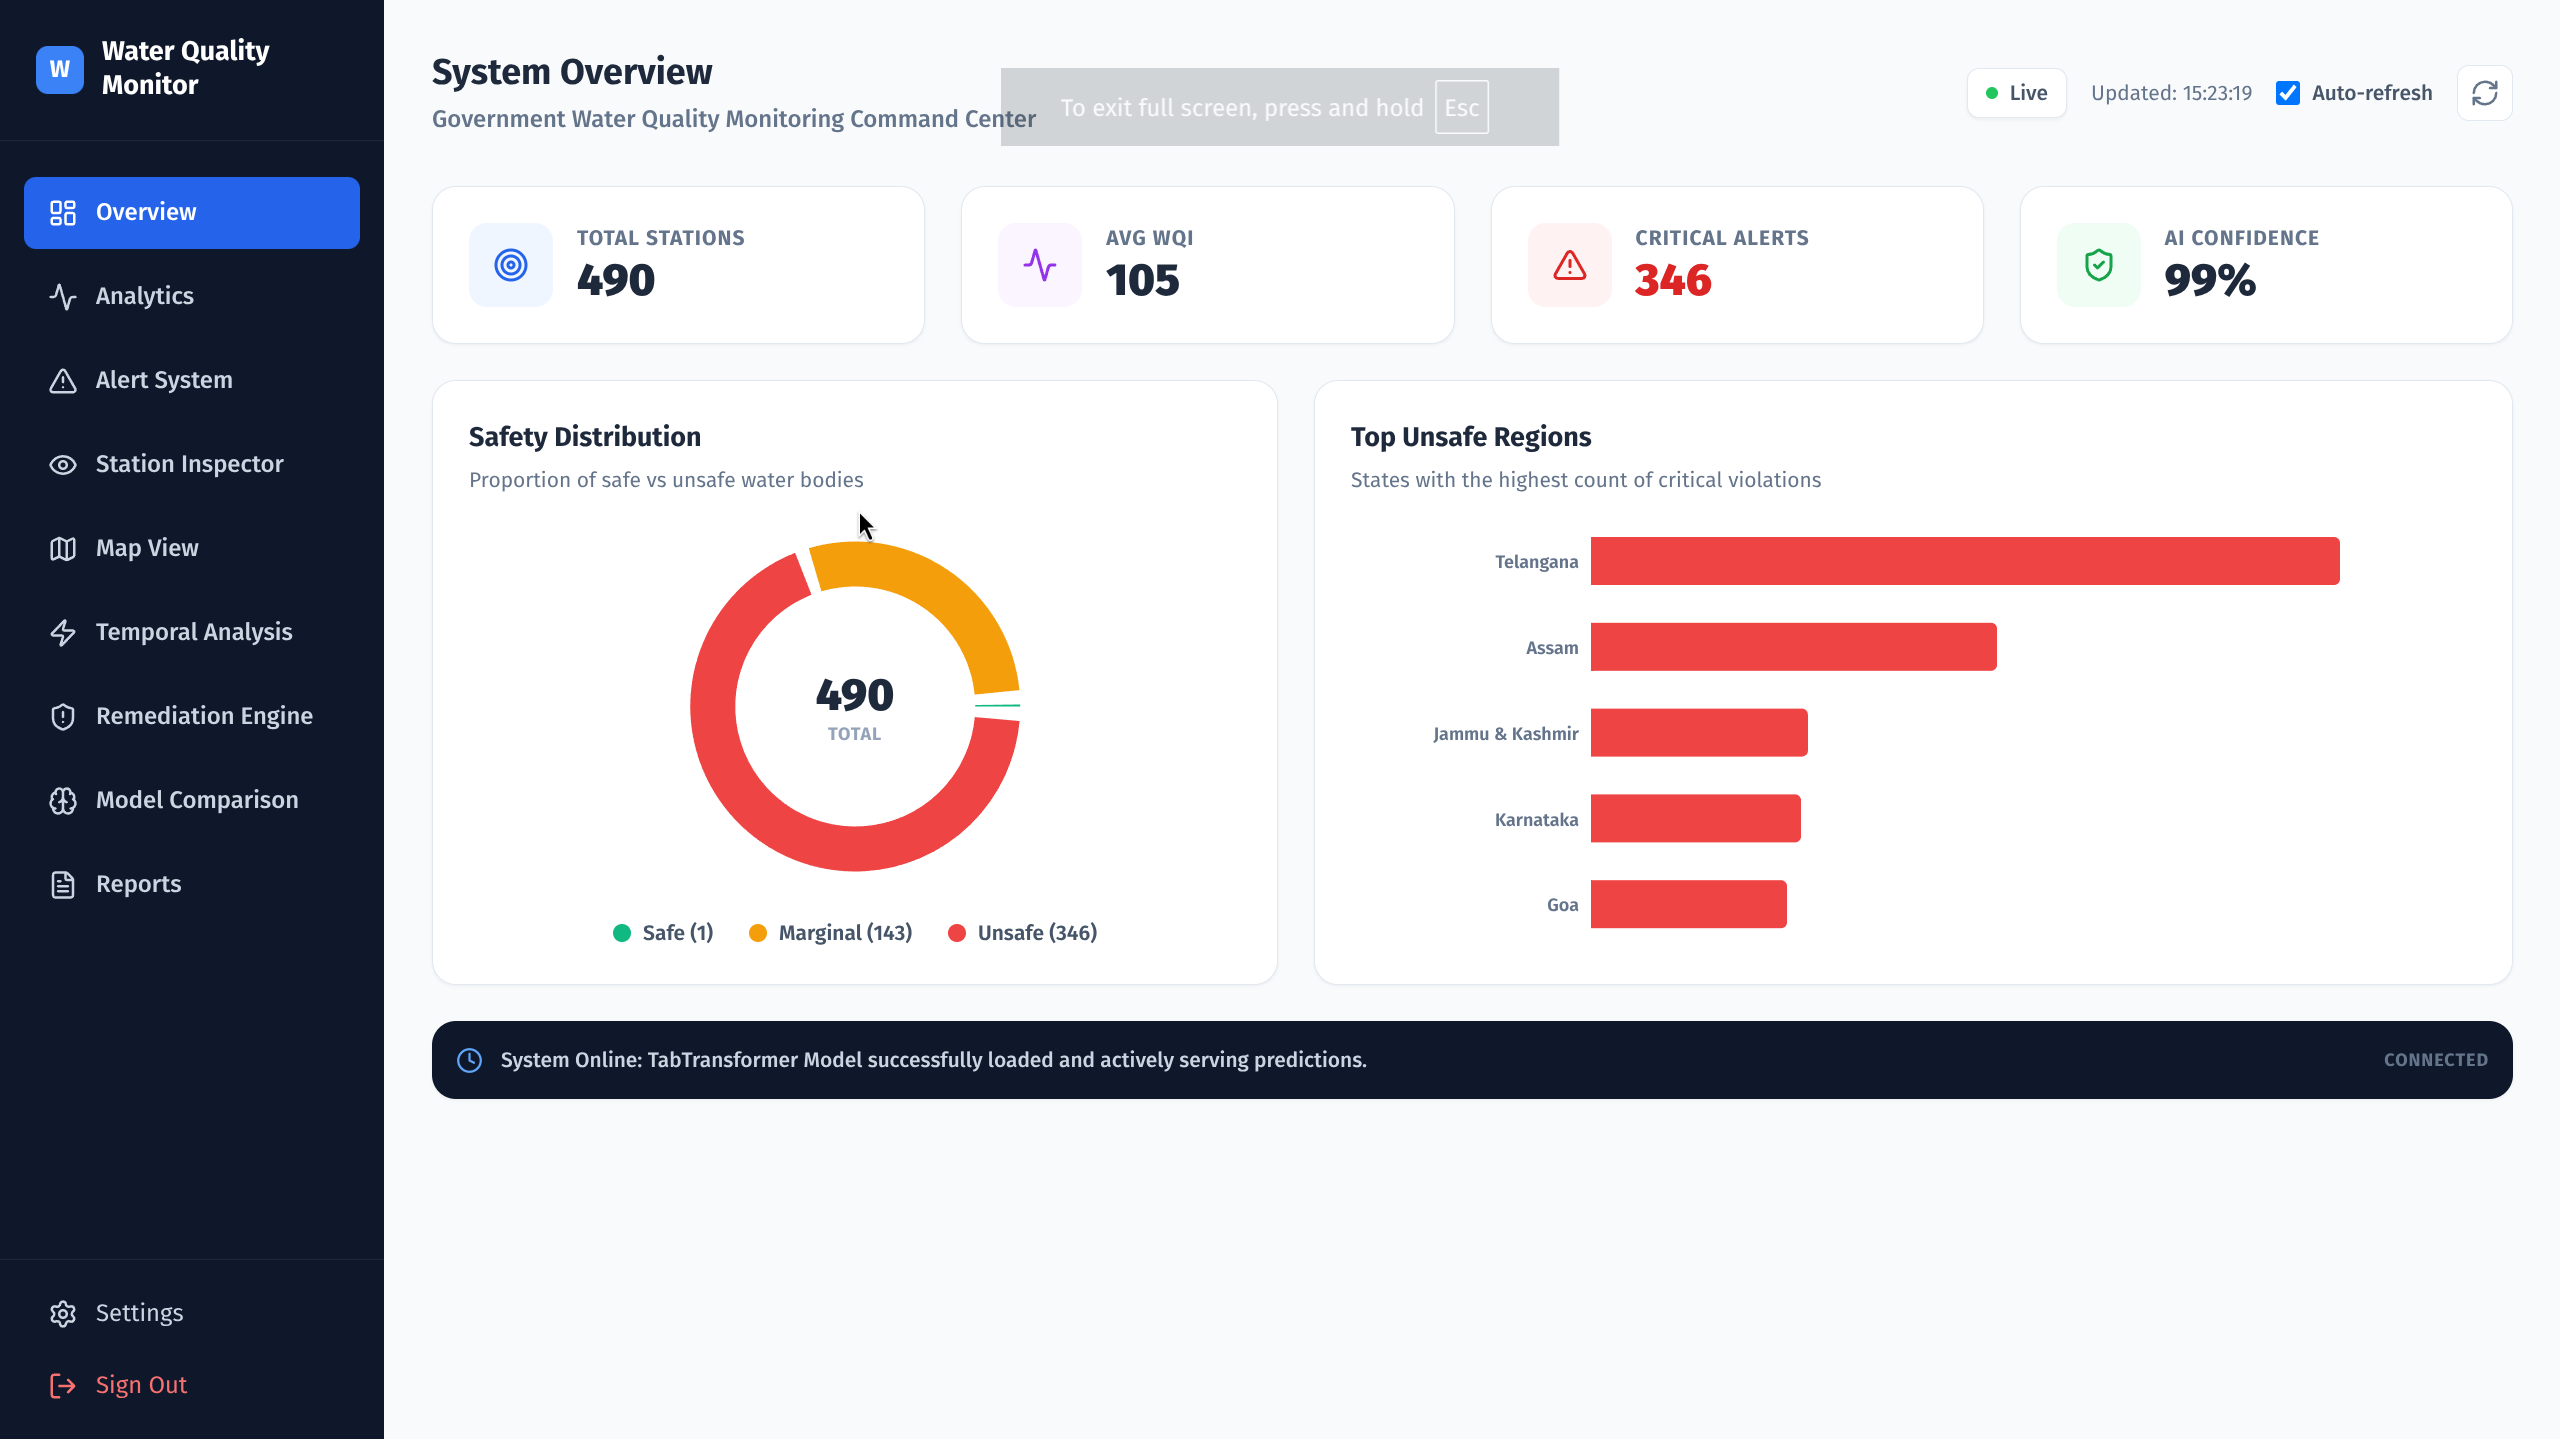
\includegraphics[width=0.96\textwidth,height=0.28\textheight,keepaspectratio]{images/overview_dashboard.png}
  \caption{System overview with station counts, water quality indicators, safety distribution, and regional alerts.}
  \label{fig:implementation-overview}
\end{figure}

\begin{figure}[H]
  \centering
  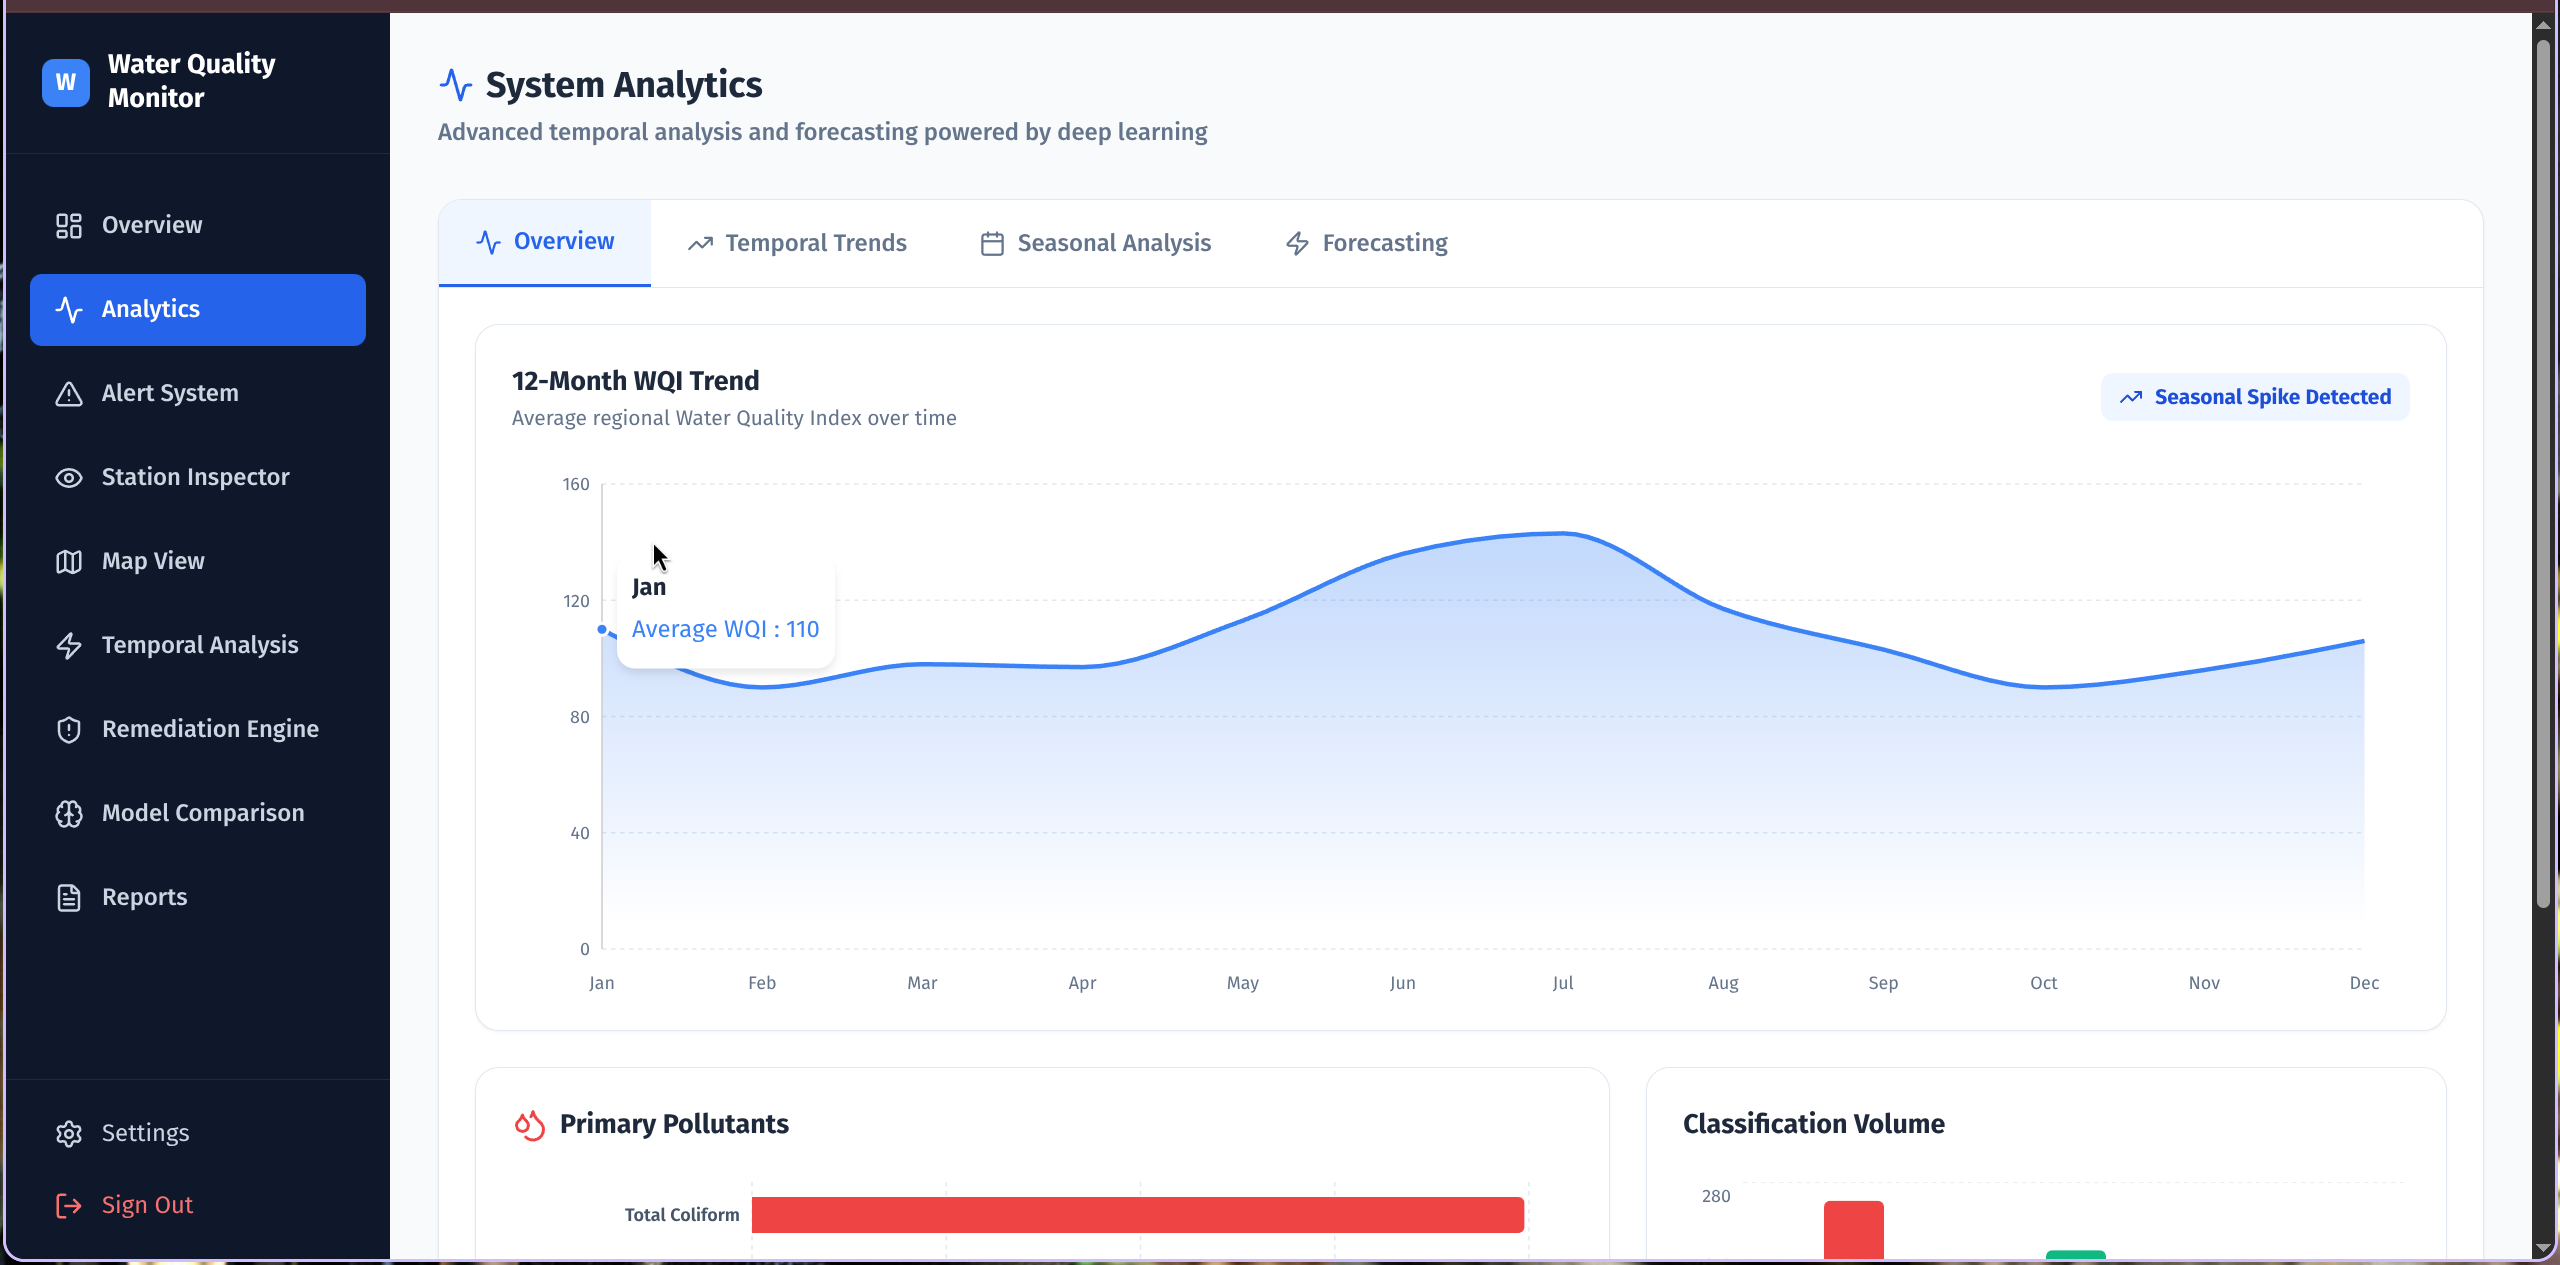
\includegraphics[width=0.96\textwidth,height=0.28\textheight,keepaspectratio]{images/analytics_dashboard.png}
  \caption{Analytics dashboard with monthly WQI trends and pollutant summaries.}
  \label{fig:implementation-analytics}
\end{figure}

\begin{figure}[H]
  \centering
  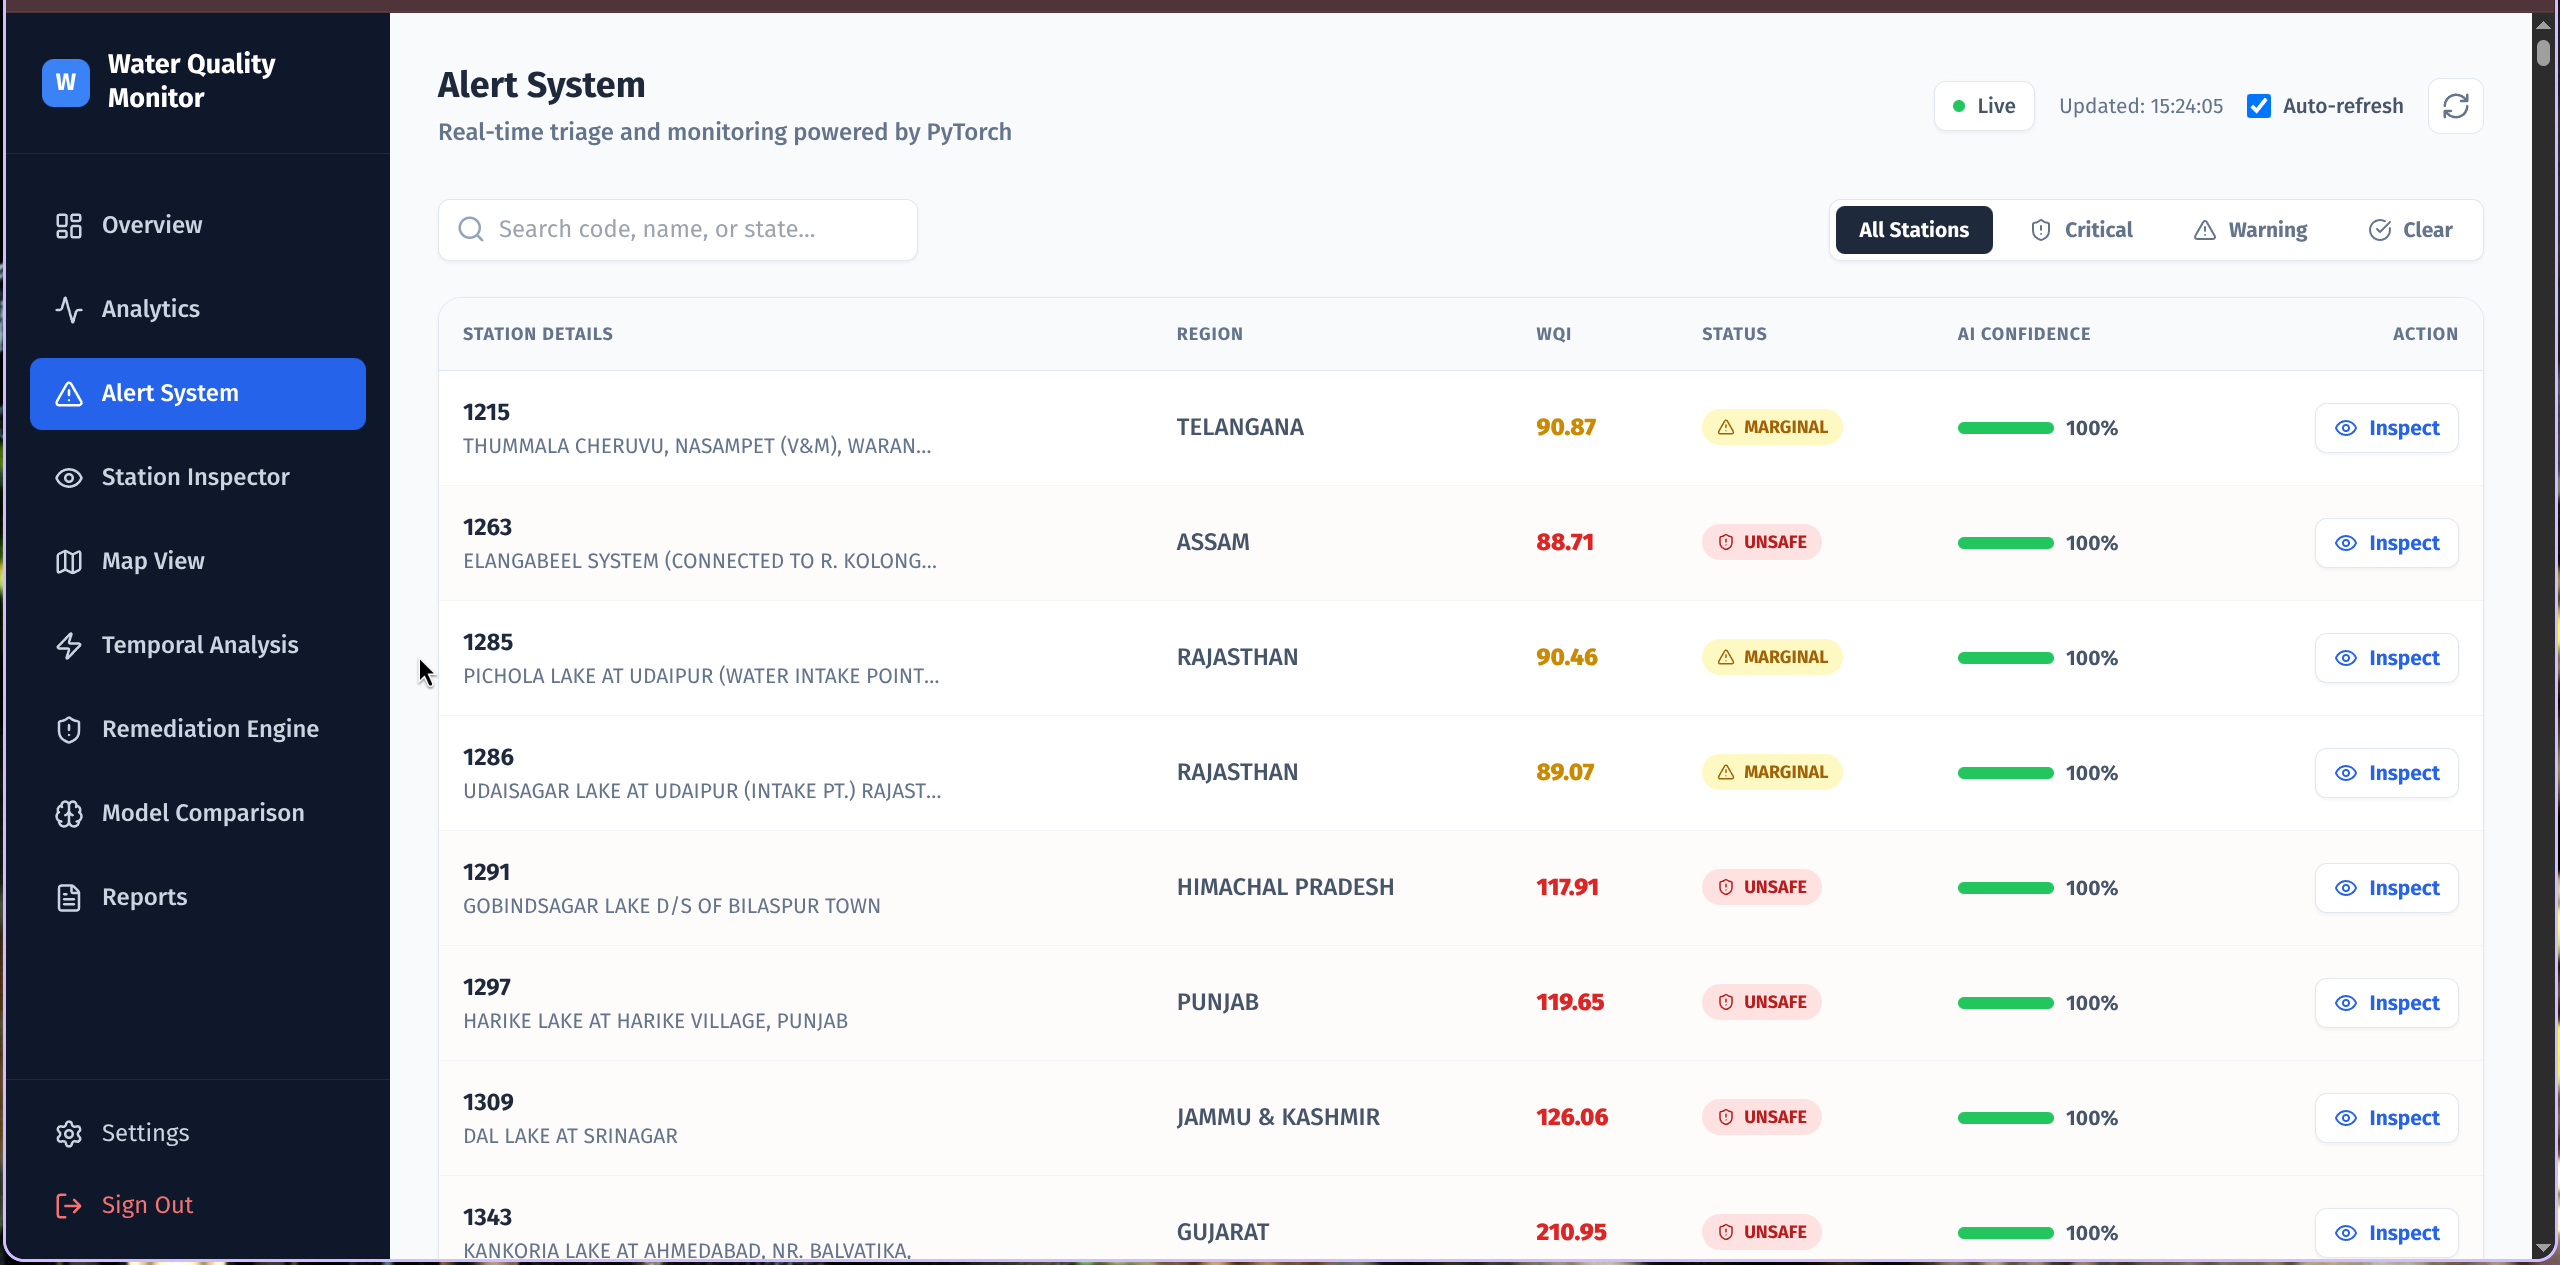
\includegraphics[width=0.96\textwidth,height=0.28\textheight,keepaspectratio]{images/alert_system_dashboard.png}
  \caption{Alert system listing stations with water quality status and model confidence.}
  \label{fig:alert-system}
\end{figure}

\begin{figure}[H]
  \centering
  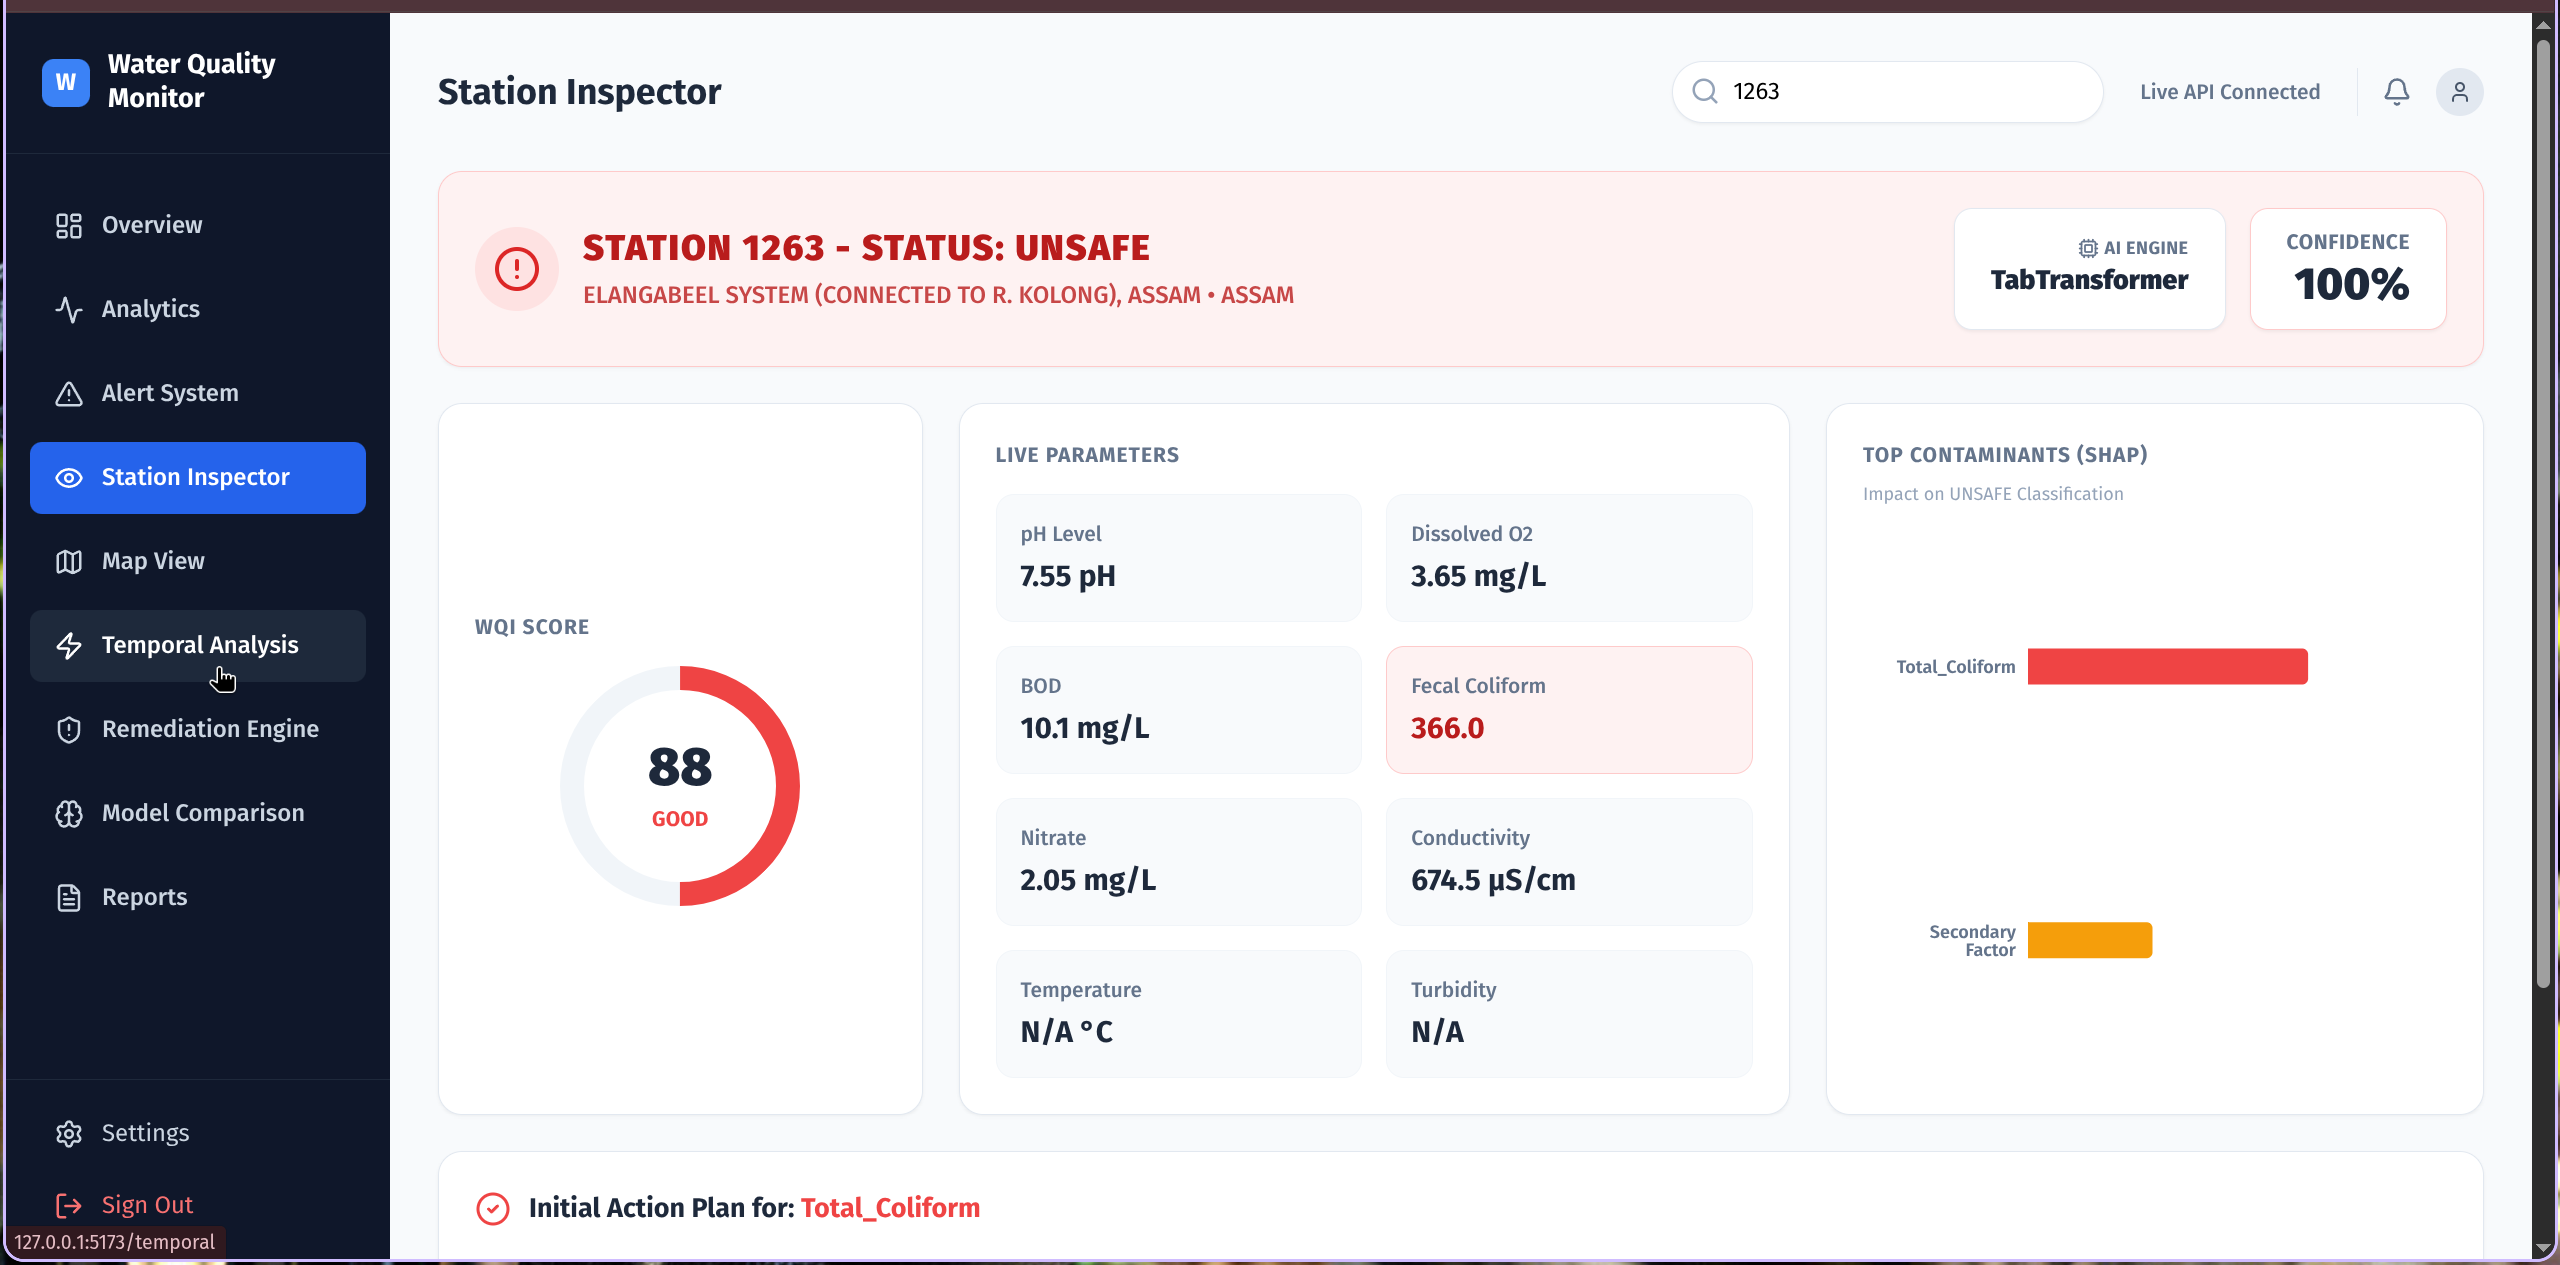
\includegraphics[width=0.96\textwidth,height=0.28\textheight,keepaspectratio]{images/station_inspector_1263_temporal_hover.png}
  \caption{Station Inspector showing unsafe status and live parameters for Station 1263.}
  \label{fig:station-inspector-temporal-hover}
\end{figure}

\begin{figure}[H]
  \centering
  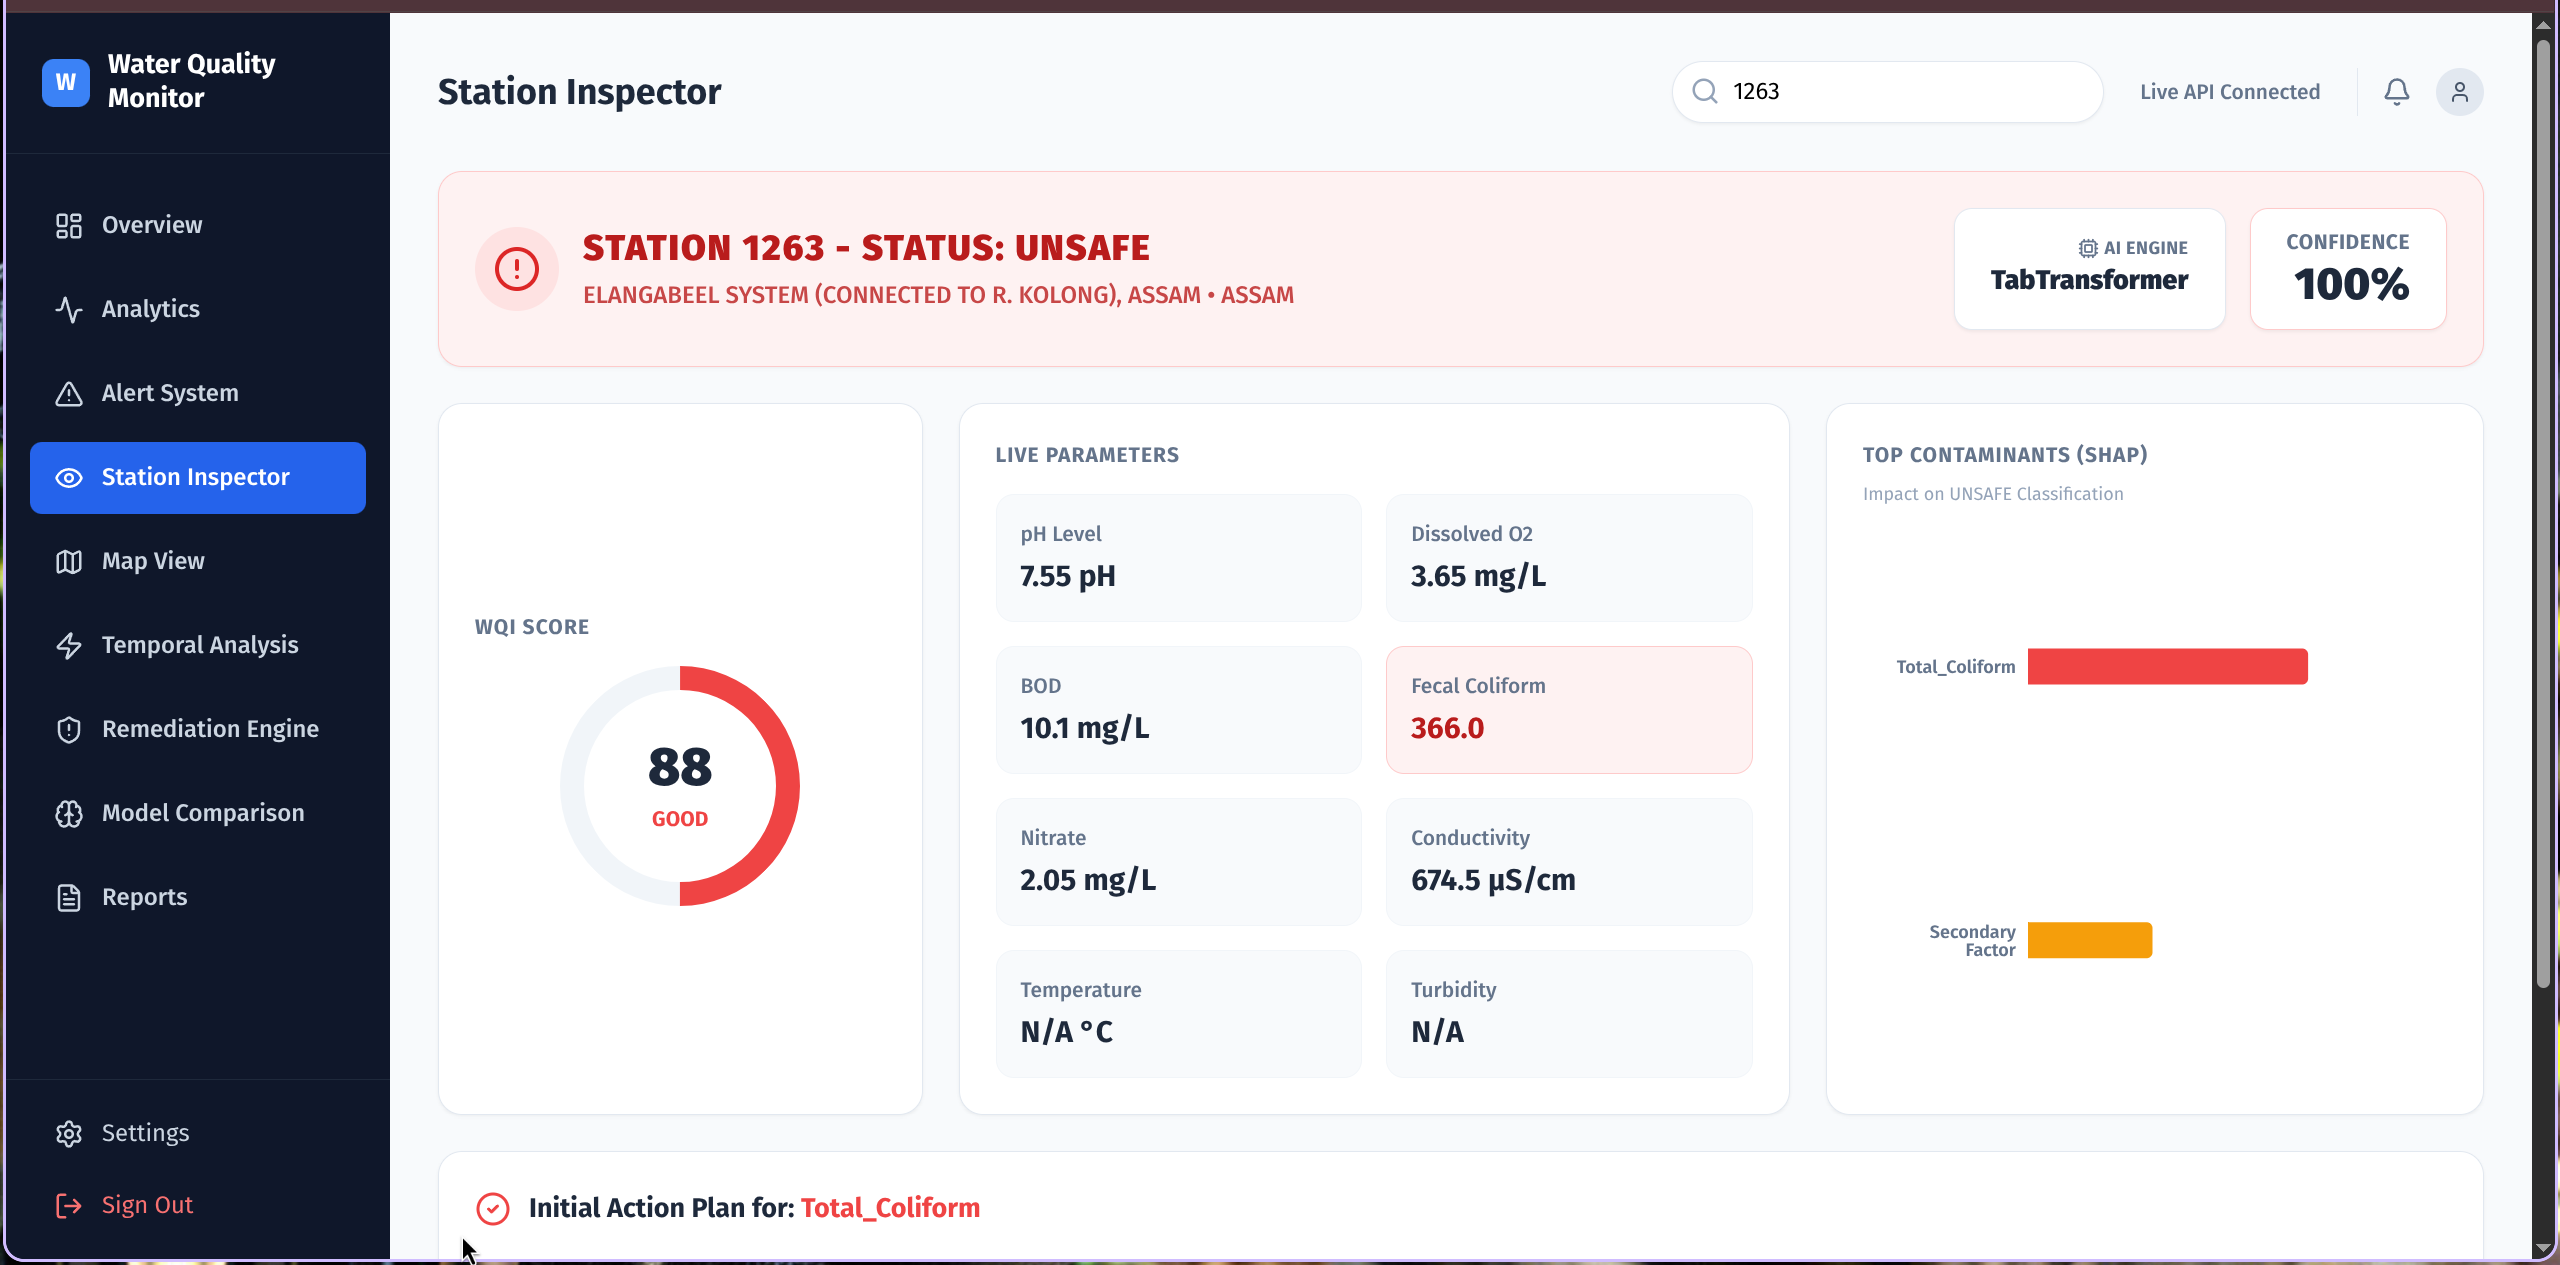
\includegraphics[width=0.96\textwidth,height=0.28\textheight,keepaspectratio]{images/station_inspector_1263_details.png}
  \caption{Station 1263 inspection view with WQI score, live parameters, and SHAP contaminant ranking.}
  \label{fig:station-inspector-details}
\end{figure}

\begin{figure}[H]
  \centering
  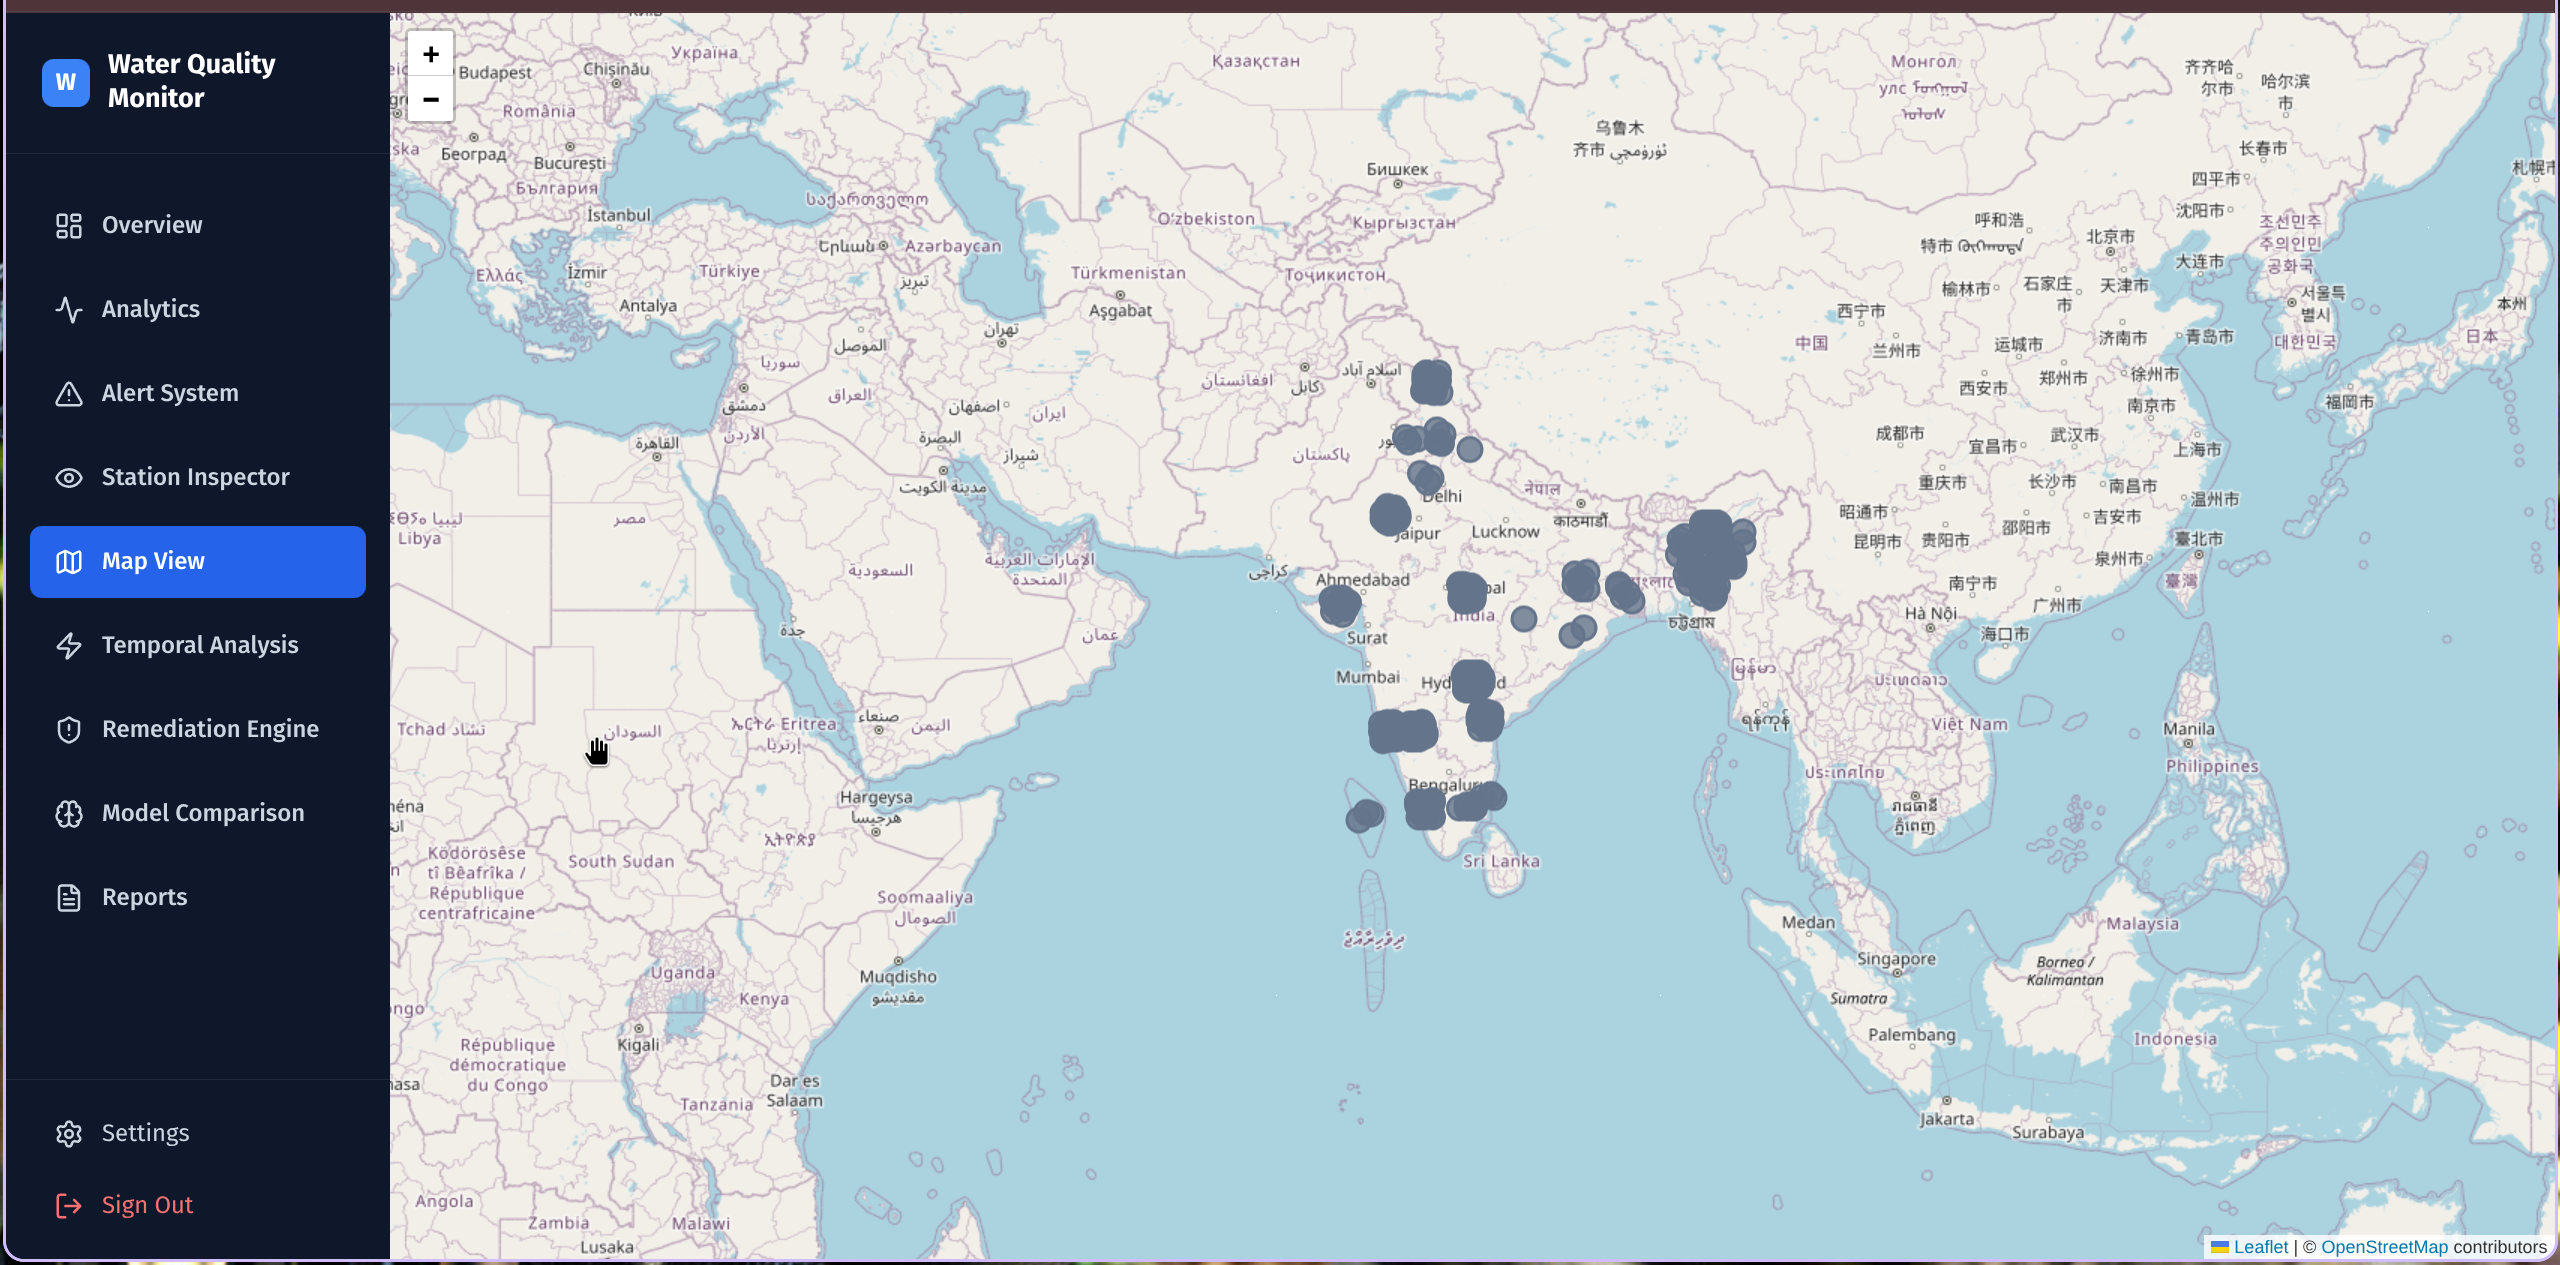
\includegraphics[width=0.96\textwidth,height=0.28\textheight,keepaspectratio]{images/station_map_dashboard.png}
  \caption{Map view locating monitored water quality stations across India.}
  \label{fig:station-map}
\end{figure}

\begin{figure}[H]
  \centering
  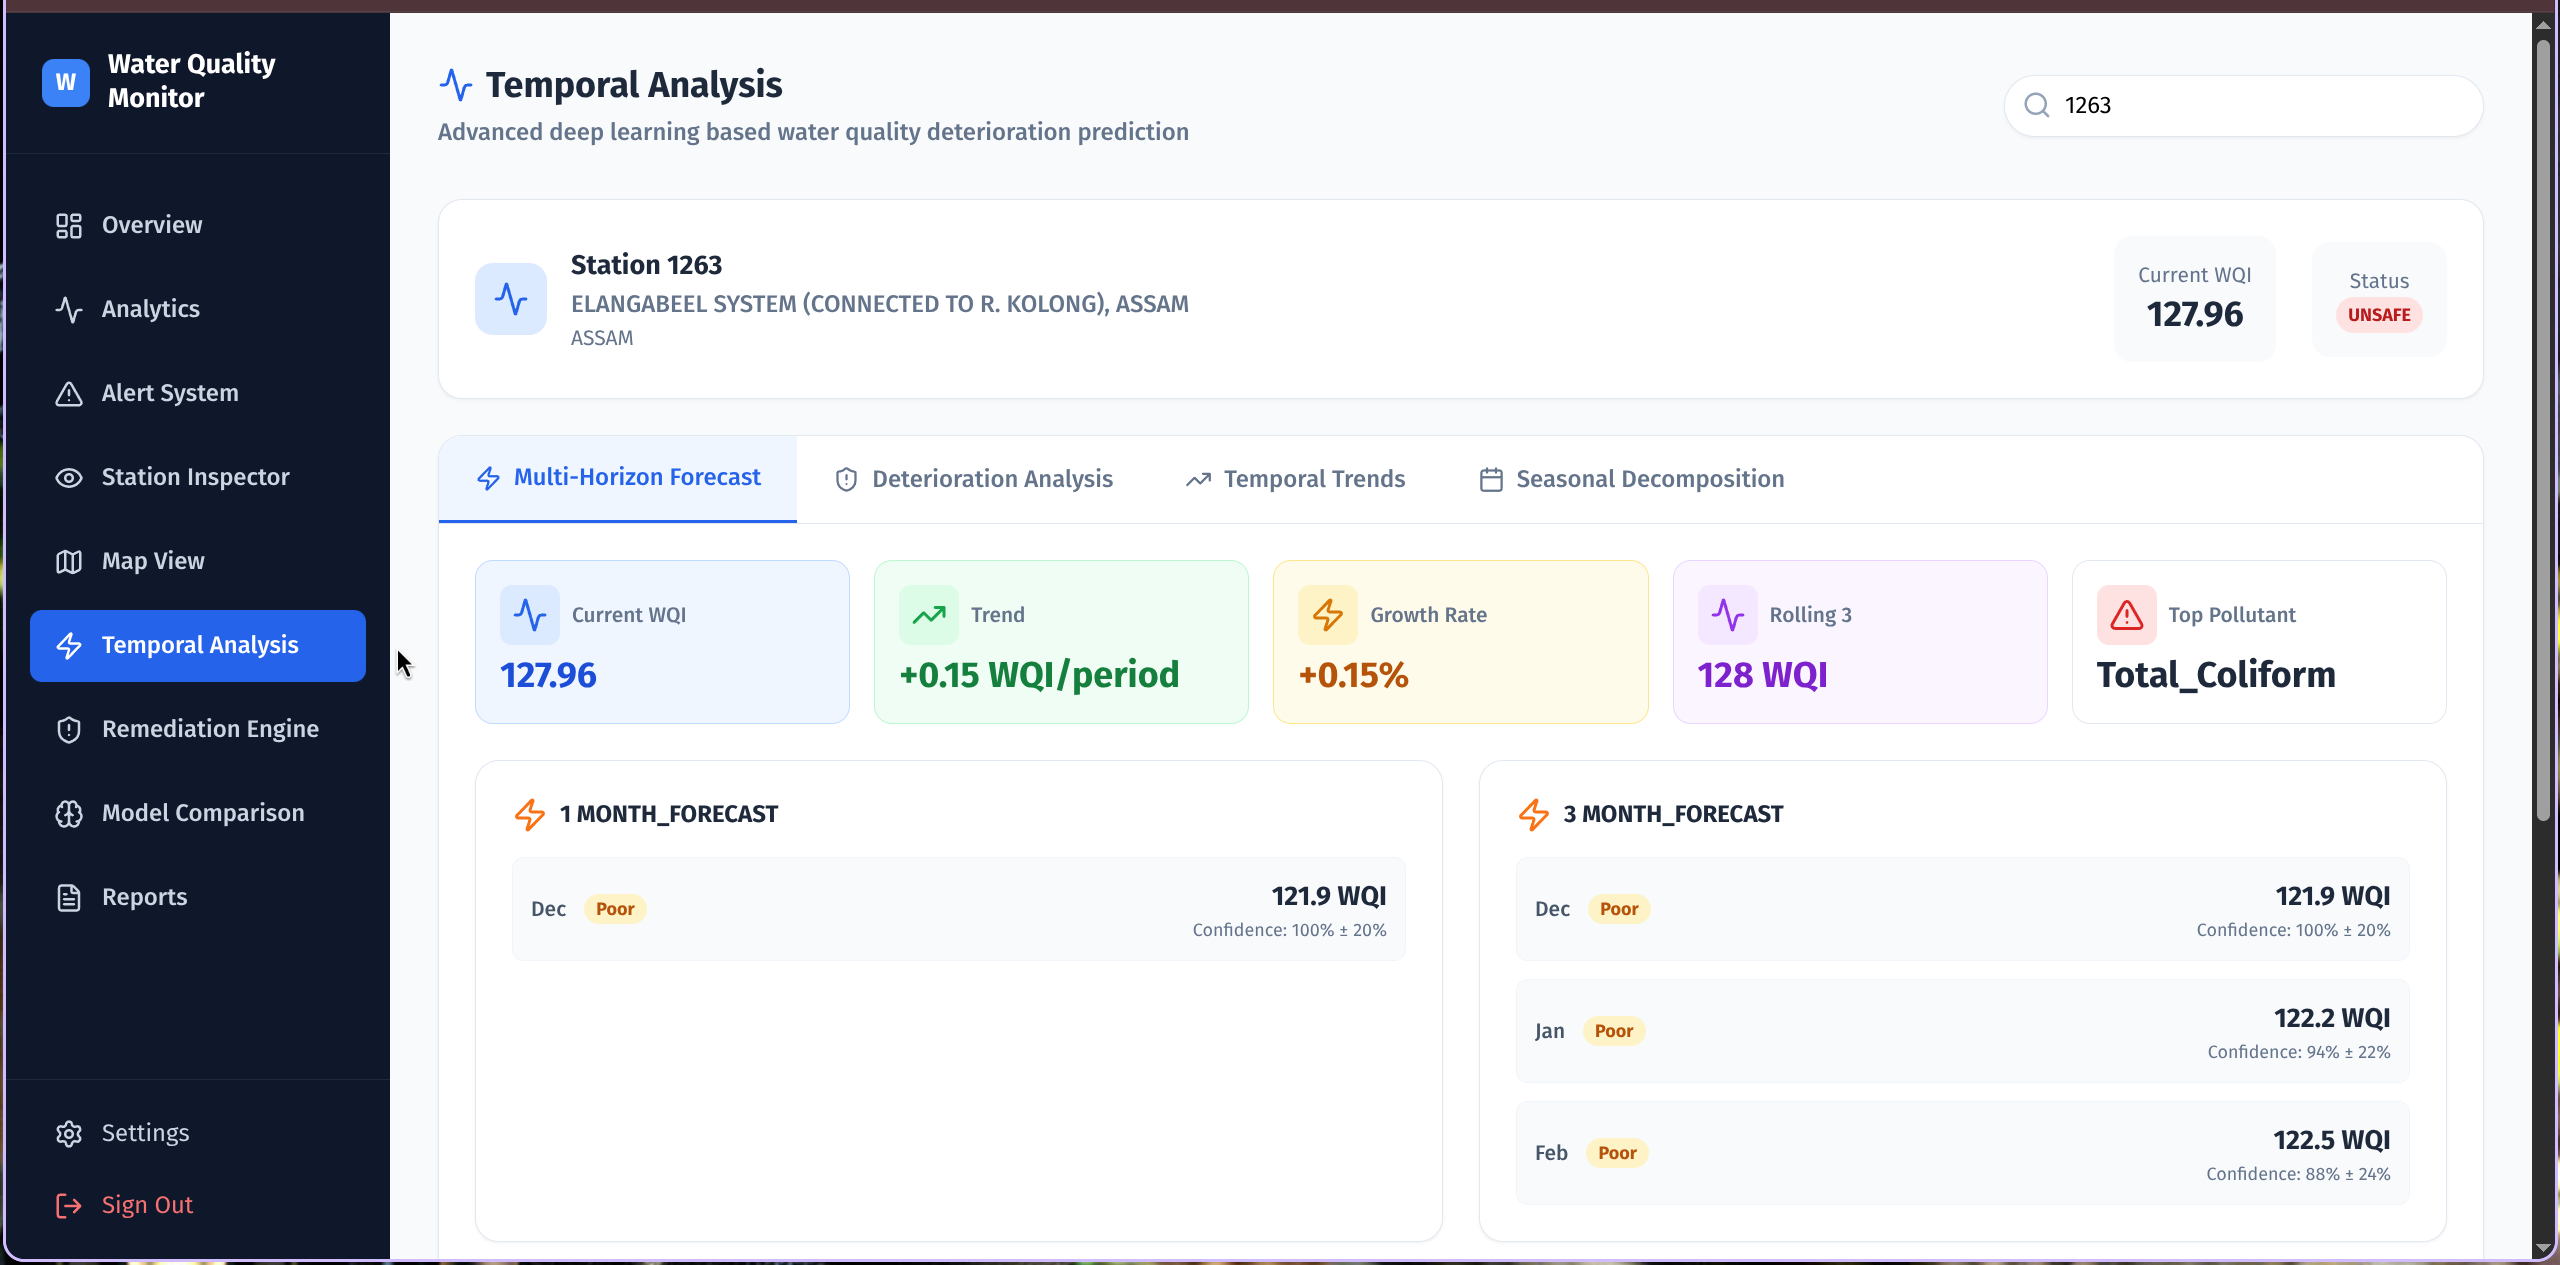
\includegraphics[width=0.96\textwidth,height=0.28\textheight,keepaspectratio]{images/temporal_analysis_dashboard.png}
  \caption{Temporal analysis view with multi-horizon forecasts and station deterioration indicators.}
  \label{fig:temporal-analysis}
\end{figure}

\begin{figure}[H]
  \centering
  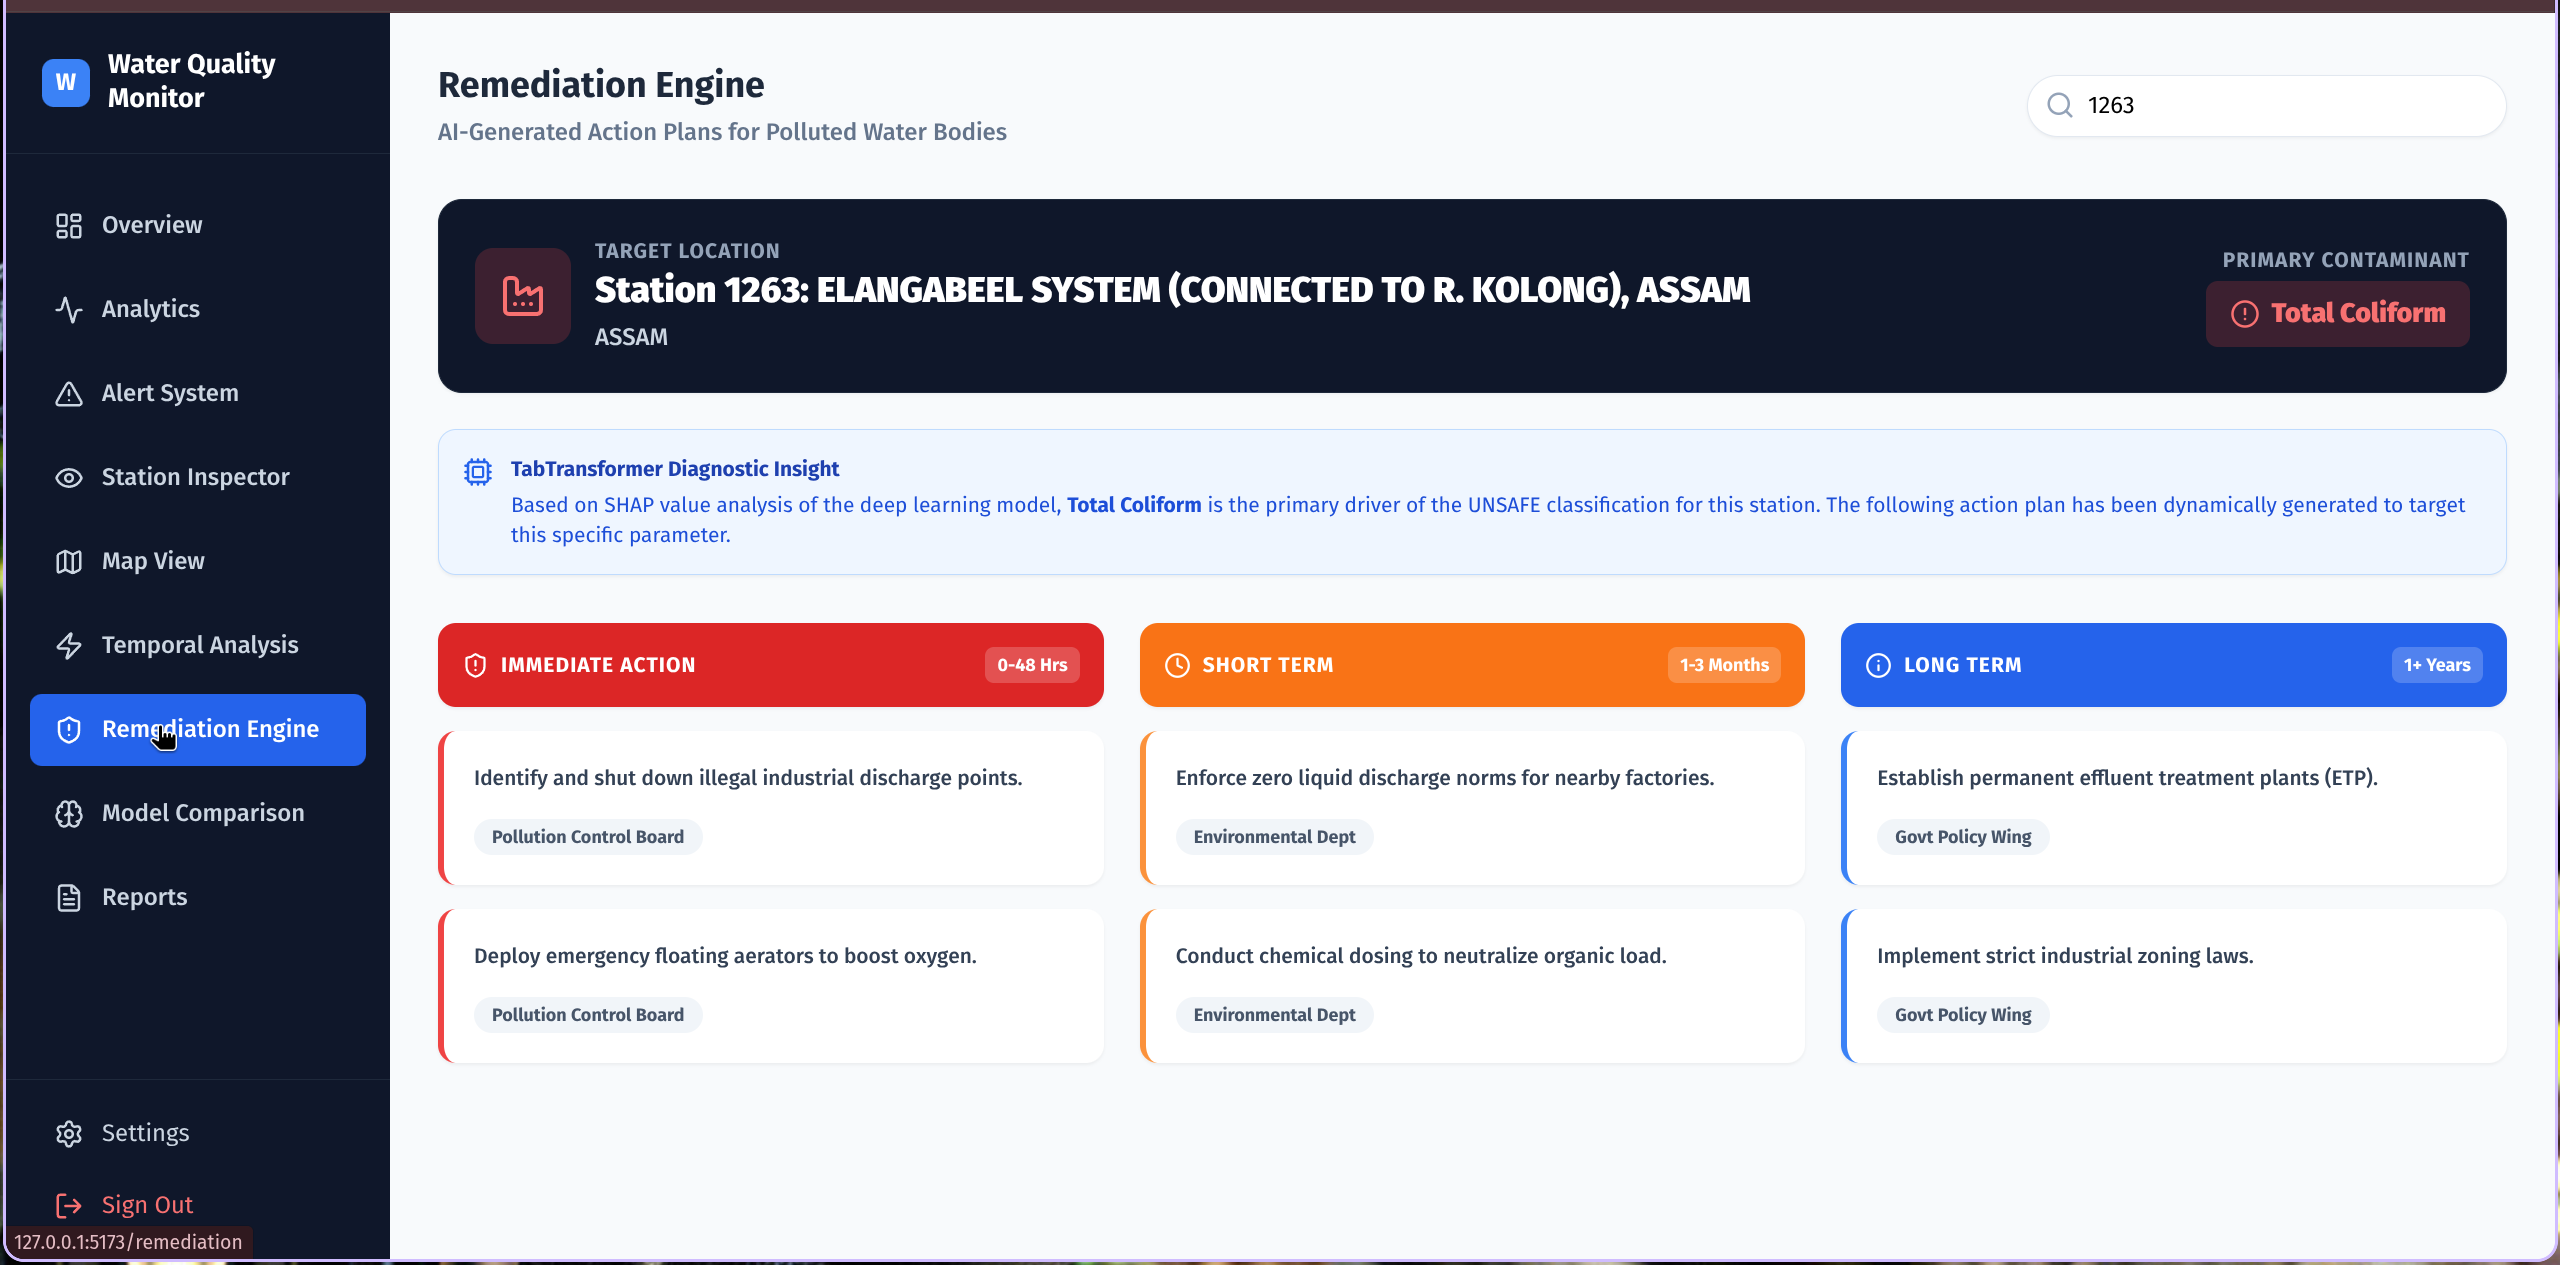
\includegraphics[width=0.96\textwidth,height=0.28\textheight,keepaspectratio]{images/remediation_engine_dashboard.png}
  \caption{Remediation Engine showing immediate, short-term, and long-term actions for Station 1263.}
  \label{fig:remediation-dashboard}
\end{figure}

\begin{figure}[H]
  \centering
  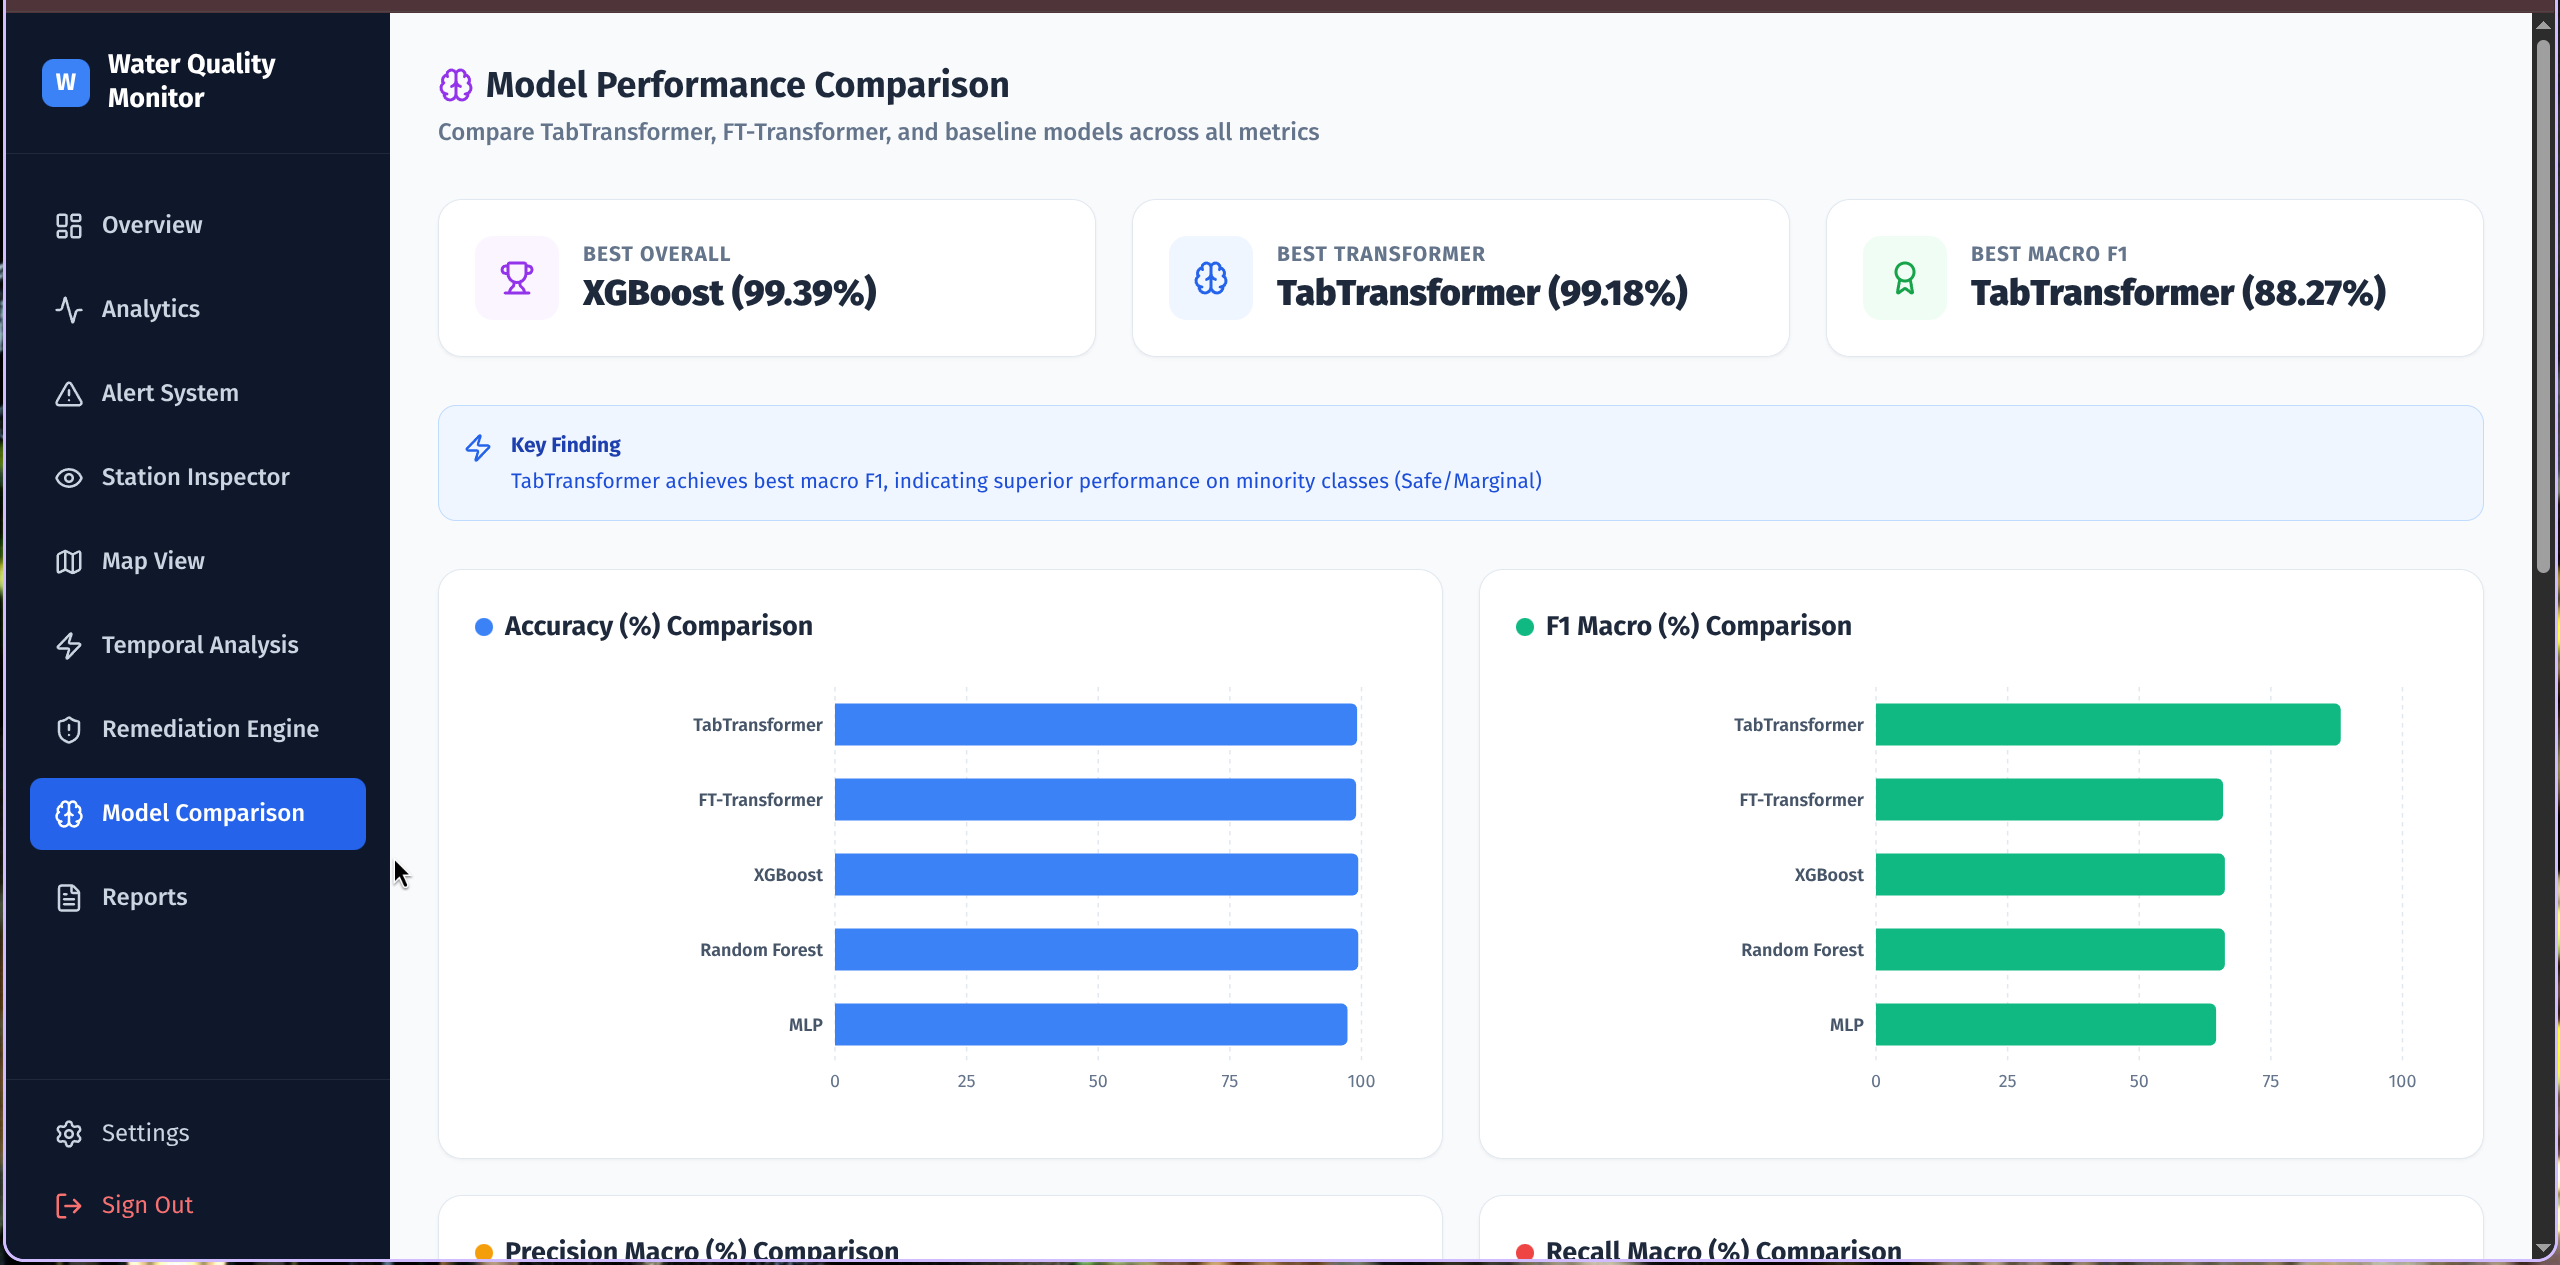
\includegraphics[width=0.96\textwidth,height=0.28\textheight,keepaspectratio]{images/model_comparison_dashboard.png}
  \caption{Model performance comparison across accuracy, macro F1, precision, and recall.}
  \label{fig:model-comparison-dashboard}
\end{figure}

\begin{figure}[H]
  \centering
  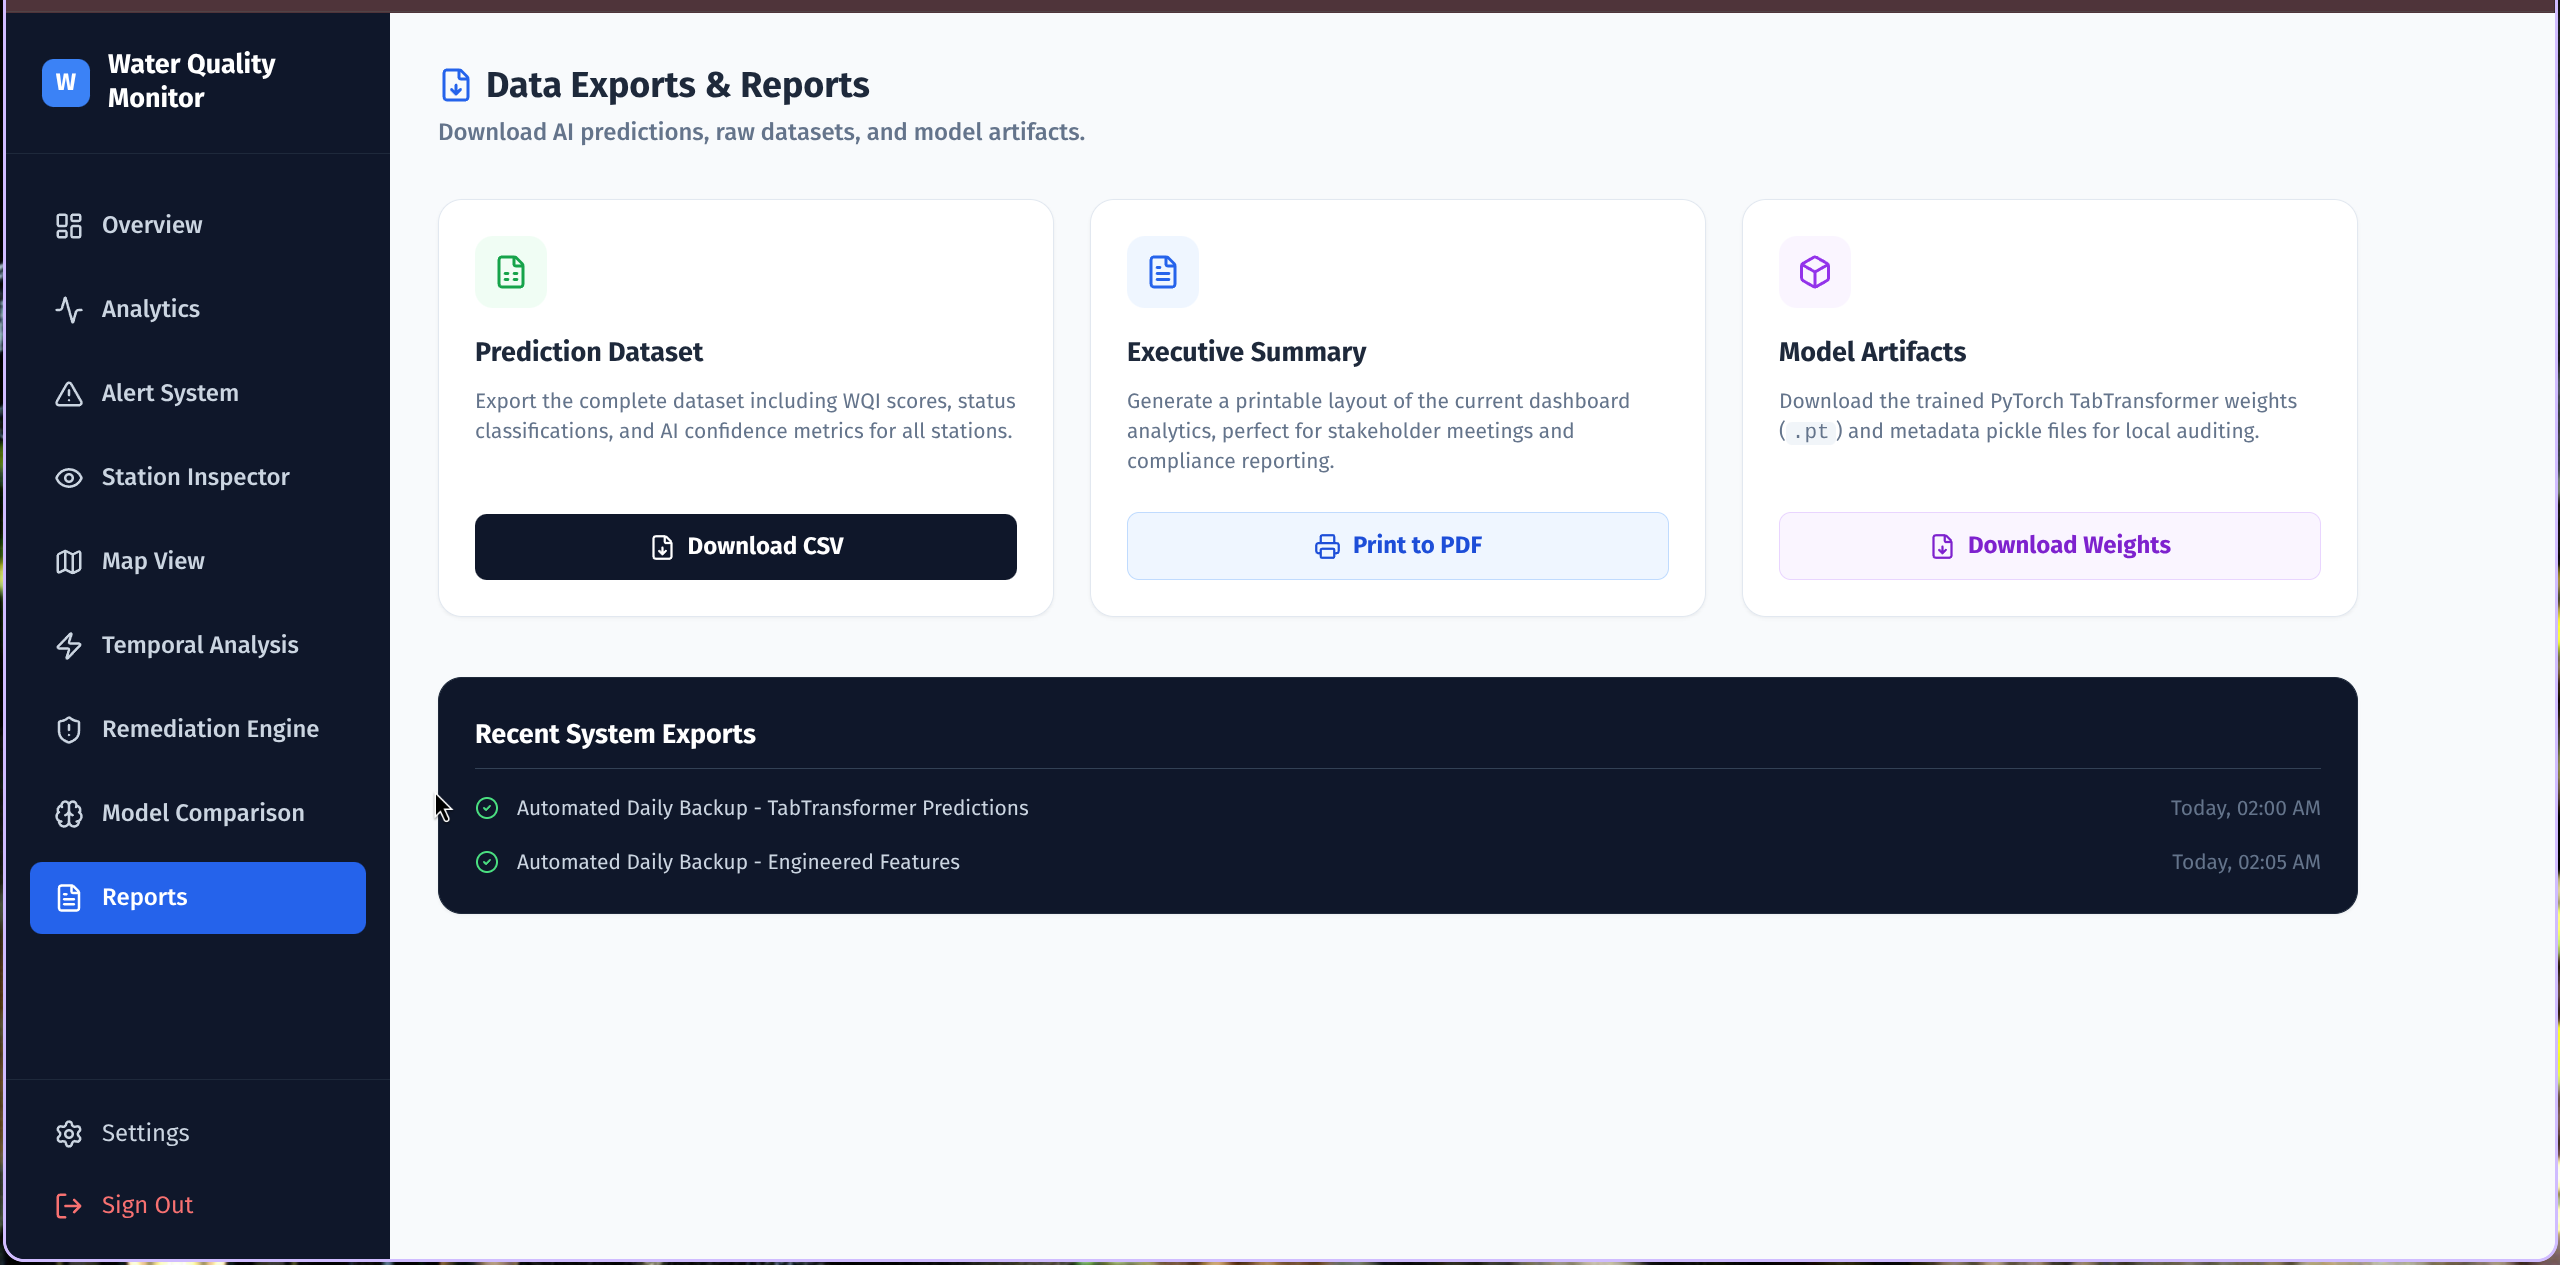
\includegraphics[width=0.96\textwidth,height=0.28\textheight,keepaspectratio]{images/reports_exports_dashboard.png}
  \caption{Reports page for exporting prediction data, executive summaries, and model artifacts.}
  \label{fig:reports-dashboard}
\end{figure}

\begin{verbatim}
# ===================== IMPORTS =====================
import pandas as pd
import numpy as np
import torch
import torch.nn as nn
import torch.nn.functional as F
from torch.utils.data import Dataset, DataLoader
from sklearn.preprocessing import StandardScaler
from sklearn.metrics import classification_report, accuracy_score
from sklearn.model_selection import train_test_split
from torch.optim import AdamW
from torch.optim.lr_scheduler import CosineAnnealingLR
import shap
import math
from scipy import signal
from scipy.interpolate import interp1d

# ===================== SETTINGS =====================
DEVICE = torch.device('cuda' if torch.cuda.is_available() else 'cpu')
SEED = 42
torch.manual_seed(SEED)
np.random.seed(SEED)

# ===================== DATA LOADING =====================
FILE_PATH = 'Water_Quality_Combined_2019_2023.xlsx'
df_raw = pd.read_excel(FILE_PATH)

# ===================== DATA CLEANING =====================
PARAM_PAIRS = {
    'Temperature': ('Temp_Min','Temp_Max'),
    'DO': ('DO_Min','DO_Max'),
    'pH': ('pH_Min','pH_Max'),
    'Conductivity': ('Conductivity_Min','Conductivity_Max'),
    'BOD': ('BOD_Min','BOD_Max'),
    'Nitrate': ('Nitrate_Min','Nitrate_Max'),
    'Fecal_Coliform': ('Fecal_Coliform_Min','Fecal_Coliform_Max'),
    'Total_Coliform': ('Total_Coliform_Min','Total_Coliform_Max'),
}

df = pd.DataFrame()
df['Year'] = df_raw['Year']
df['Station_Code'] = df_raw['Station_Code']
df['State'] = df_raw['State']

for p,(lo,hi) in PARAM_PAIRS.items():
    df[p] = (df_raw[lo].astype(float) + df_raw[hi].astype(float)) / 2

for col in PARAM_PAIRS:
    df[col] = df.groupby('Station_Code')[col].transform(lambda x: x.fillna(x.median()))
    df[col] = df[col].fillna(df[col].median())

# ===================== BIS LABEL =====================
BIS = {
    'pH': ('range',6.5,8.5,9.2),
    'DO': ('higher',6.0,4.0,None),
    'BOD': ('lower',2.0,5.0,None),
    'Nitrate': ('lower',45.0,100.0,None),
    'Conductivity': ('lower',750.0,3000.0,None),
    'Fecal_Coliform': ('lower',2.2,500.0,None),
    'Total_Coliform': ('lower',10.0,500.0,None),
}

def classify_param(v, rule):
    if pd.isna(v): return 0
    if rule[0]=='higher':
        return 0 if v>=rule[1] else (1 if v>=rule[2] else 2)
    if rule[0]=='range':
        return 0 if rule[1]<=v<=rule[2] else (1 if rule[1]<=v<=rule[3] else 2)
    return 0 if v<=rule[1] else (1 if v<=rule[2] else 2)

def classify_sample(row):
    return max(classify_param(row[p],BIS[p]) for p in BIS)

df['BIS_Class'] = df.apply(classify_sample,axis=1)

# ===================== WQI =====================
WQI_LIMITS = {'BOD':5.0,'Nitrate':100.0,'DO':4.0}

def compute_wqi(row):
    total = 0
    count = 0
    for p,lim in WQI_LIMITS.items():
        if pd.isna(row[p]): continue
        total += (row[p]/lim)*100
        count += 1
    return total/count if count>0 else np.nan

df['WQI'] = df.apply(compute_wqi,axis=1)

# ===================== FEATURE ENGINEERING =====================
df = df.sort_values(['Station_Code','Year'])

df['WQI_Lag1'] = df.groupby('Station_Code')['WQI'].shift(1)
df['WQI_Lag1'] = df['WQI_Lag1'].fillna(df['WQI'].median())

df['WQI_Rolling3'] = df.groupby('Station_Code')['WQI'] \
                        .transform(lambda x: x.rolling(3,min_periods=1).mean())

station_avg = df.groupby('Station_Code')['WQI'].mean()
df['Station_Avg_WQI'] = df['Station_Code'].map(station_avg)

state_avg = df.groupby('State')['WQI'].mean()
df['State_Avg_WQI'] = df['State'].map(state_avg)

# ===================== TRAIN TEST =====================
FEATURES = [
    'Temperature','DO','pH','Conductivity','BOD','Nitrate',
    'Fecal_Coliform','Total_Coliform',
    'WQI','WQI_Lag1','WQI_Rolling3',
    'Station_Avg_WQI','State_Avg_WQI'
]

X = df[FEATURES].values.astype(np.float32)
y = df['BIS_Class'].values

scaler = StandardScaler()
X = scaler.fit_transform(X)

X_train,X_test,y_train,y_test = train_test_split(X,y,test_size=0.2)

# ===================== DATASET =====================
class WaterDataset(Dataset):
    def __init__(self,X,y):
        self.X=torch.tensor(X,dtype=torch.float32)
        self.y=torch.tensor(y,dtype=torch.long)
    def __len__(self): return len(self.y)
    def __getitem__(self,i): return self.X[i],self.y[i]

train_loader = DataLoader(WaterDataset(X_train,y_train),batch_size=64,shuffle=True)
test_loader  = DataLoader(WaterDataset(X_test,y_test),batch_size=64)

# ===================== TABTRANSFORMER =====================
class TabTransformer(nn.Module):
    def __init__(self,n_features,n_classes):
        super().__init__()
        self.embed = nn.Linear(1,64)
        self.pos = nn.Parameter(torch.randn(1,n_features,64))

        encoder = nn.TransformerEncoderLayer(d_model=64,nhead=8,batch_first=True)
        self.transformer = nn.TransformerEncoder(encoder,4)

        self.fc = nn.Sequential(
            nn.Linear(64*n_features,256),
            nn.ReLU(),
            nn.Linear(256,n_classes)
        )

    def forward(self,x):
        x=x.unsqueeze(-1)
        x=self.embed(x)+self.pos
        x=self.transformer(x)
        x=x.flatten(1)
        return self.fc(x)

model = TabTransformer(len(FEATURES),3).to(DEVICE)

# ===================== TRAINING =====================
optimizer = AdamW(model.parameters(),lr=3e-4)
scheduler = CosineAnnealingLR(optimizer,T_max=20)
criterion = nn.CrossEntropyLoss()

for epoch in range(20):
    model.train()
    for xb,yb in train_loader:
        xb,yb = xb.to(DEVICE),yb.to(DEVICE)
        optimizer.zero_grad()
        pred=model(xb)
        loss=criterion(pred,yb)
        loss.backward()
        optimizer.step()
    scheduler.step()

# ===================== EVALUATION =====================
model.eval()
with torch.no_grad():
    preds = model(torch.tensor(X_test).to(DEVICE)).argmax(1).cpu().numpy()

print("Accuracy:",accuracy_score(y_test,preds))
print(classification_report(y_test,preds))

# ===================== SHAP =====================
explainer = shap.Explainer(model, torch.tensor(X_train))
shap_values = explainer(torch.tensor(X_test))

# ===================== CONFIDENCE =====================
def bootstrap_confidence(model,X,n=30):
    outputs=[]
    for _ in range(n):
        pred=model(X).argmax(1)
        outputs.append(pred.cpu().numpy())
    return np.mean(outputs,axis=0)

confidence = bootstrap_confidence(model,torch.tensor(X_test).to(DEVICE))
\end{verbatim}

%=============================================================================
\end{document}
%=============================================================================
